%# -*- coding: utf-8 -*-
% !TEX encoding = UTF-8 Unicode
\RequirePackage{fixltx2e}
\documentclass[aps,pre,12pt,preprint,onecolumn,showpacs,showkeys,UTF8]{revtex4-1}
\usepackage{ctex}
\usepackage{mathrsfs}
\usepackage{setspace,dcolumn}
\usepackage{subfigure}
\usepackage{graphicx,psfrag,epsfig}
\usepackage[font=small,format=plain,labelfont=bf,textfont=it,justification=raggedright,singlelinecheck=false]{caption}
\usepackage{amsmath,amsfonts,amssymb,amsthm,bm,upgreek}
\usepackage{geometry}
\usepackage[mathscr]{eucal}
\usepackage{titlesec}
\usepackage{tabularx}
\titleformat{\section}{\bf\fangsong\zihao{4}}{\thesection}{0.75em}{}
\geometry{top=2.54cm,bottom=2.54cm,left=3cm,right=3cm}
\renewcommand\appendixname{附录}
\renewcommand\abstractname{}%摘要
\renewcommand\tablename{表}
\renewcommand\figurename{图}
\makeatletter
\def\@keys@name{\songti\zihao{-4}{\bf 关键词:}}
\def\Received@name{\zihao{-5}{接收} }
\def\Revised@name{\zihao{-5}{修订} }
\def\Accepted@name{\zihao{-5}{采纳} }
\def\Published@name{\zihao{-4}{发表} }
\makeatother
\linespread{1.6}
\renewcommand{\labelenumi}{\alph{enumi}.}
\leftmargini=20mm

\begin{document}

\title{\bf\heiti\zihao{3}利用电子衍射测量Cu,Ag,Sn,Si的晶格常数\vspace{15mm}}
\author{\fangsong 乔颢\vspace{2mm}}
\affiliation{\songti\zihao{-4}北京大学物理学院2011级2班~~~~学号:1100011354 \vspace{2mm}}
\keywords{电子衍射,晶格常数,固体,指标化处理}
\email{1993422qsh@gmail.com; 18600200672}
\begin{abstract}
	\vspace{10mm}
	\begin{spacing}{1.5}
		\songti\zihao{-4}
		本实验利用透射电子显微镜,观测了Au,Ag,Cu,Sn,Si元素晶体的衍射图样,并且利用Au进行定标,使用指标化的处理方法计算出来了其他四种元素的晶格常数。分别为$4.1\AA$,$3.6\AA$,$6.5\AA$,$5.7\AA$。其中Si为单晶体,其他则为多晶体。
	\end{spacing}
\end{abstract}

\maketitle

\section{引言}
在普朗克和爱因斯坦关于光的微粒性理论成功的基础上,德布罗意在1924年提出了微观粒子也具有波粒二相性的假说,即对于具有能量E的微观粒子,其也具有波动的性质,其波长和频率$\mu$的关系与光波类似,可以得到其波长为:
\begin{equation}
	\lambda=\frac{h}{p}=\frac{h}{\sqrt{2meV}}
\end{equation}

而在1927年戴维孙和革末实验了电子打在镍单晶上得到了和X光衍射一样的现象。这次实验证明了德布罗意的假设,为量子力学打下了基础,同时也建立起来了一种研究物质性质的方法即为电子衍射。

相对于X光而言,电子束可以达到很高的加速速度,从而使得波长变得很短,能更合适的观察到衍射角。这样能够更方便的研究晶体的几何关系。同时由于电子在物质中的穿透深度很小,所以其更适用于研究微晶,表面和薄膜的晶体结构。对于低能的电子,样品只有表面的几层电子对衍射图像有贡献,所以低能电子已经成为表面结构分析的重要手段。

透射电子显微镜(TEM)通过电子光学的手段对电子加速,聚焦并使其轰击带测样品,得到带测样品的衍射图样。本次实验就是使用透射电子显微镜观察并测定铜,银,锡,硅的电子衍射图样,并由此计算出其对应的晶格常数。这个实验的目的是要求掌握电子衍射的运动学理论,并用其研究单晶体和多晶体的衍射现象。\cite{Book}

\section{实验}
\subsection{实验装置}
\begin{enumerate}
	\item 透射电子显微镜。\\透射电子显微镜由顶端灯丝和电子枪产生并加速电子形成电子束,通过磁透镜(利用环形磁场对电子束进行约束聚焦,功能上类似于透镜对于光的作用)的调整打入带测样品,并经过物镜目镜的放大以及光阑的约束等等成像到屏幕上并由荧光装置现实出来。其整体结构复杂,并且需要工作在基本真空的环境下以避免空气中的灰尘对于电子束的影响等。所以透射电子显微镜是一套极其复杂的大型仪器。
	\item 透射电镜辅助系统。\\ 因为透射电子显微镜工作需要许多复杂的条件,所以有一整套辅助系统对电镜提供支持。主要有提供电流的高压直流电源,市电稳压模块。提供真空的扩散泵和为扩散泵提供低压的真空泵。以及维持系统和磁透镜稳定性的散热系统等。本实验中的电镜处于常年工作状态,所以其可能也有一定的后备电源系统(UPS)等。
	\item 透射电镜控制台。\\控制台为操作人员提供了方便快捷的操作体验,简化了原来十分复杂的调整操作。同时其也承担着协调各个系统之间的关系的作用,例如当真空度不足时就不会为灯丝加上电流以防其烧坏,当外部真空泵失效的时候会停止扩散泵的工作防止其被压强差损坏等等。同时控制台也提供了照相或者CCD的一系列设备以提供数据的采集。本实验中电镜是使用的照相的方法收集数据。
	\item 样品。\\本实验的样品是使用真空蒸镀的方法将金属蒸镀到含孔的网上,只有足够薄的样品才不会影响到电子的通透性所以样品需要足够的薄。对于硅(Si)则是观察的纯度很高的单晶硅的边缘部分(边缘采用特殊工艺刻蚀出来,十分的薄)。
\end{enumerate}

\subsection{实验步骤}

将样品装入样品台并将其插入电镜,等待真空度达标后打开灯丝,发射160keV的电子束,调整透镜的放大倍数为最低,移动样品台,使得电子书打在样品上。调整电子束的位置使得亮度合适并且光斑中心在屏幕的正中。调整聚焦使得像清晰。随后逐步增加放大倍数并且调整样品位置,光斑位置,光斑大小,聚焦。直至放大倍数为10万倍,这时候应该能看到清晰的样品的结构。

将电镜的工作模式切换到衍射模式,同时调整亮度以及聚焦使得到一张清晰同时亮度适中的衍射图像。利用控制台的照相模式将图片曝光到胶片上。切换样品,重复上述工作,得到带测样品以及Au的衍射图样。

测量单晶硅的时候应该注意到选取的位置应该是边缘十分薄的地方,同时合理的调整样品的倾斜角度使之出现六边形的点阵,并且亮度相对均匀。

测量完成后在暗室中对胶片进行定影,显影,烘干的操作。根据定影液显影液的质量适当的调整定影显影时间,最后得到一系列清晰的照片并进行接下来的数据处理。

\section{数据分析及讨论}

\begin{figure}[h]
	\begin{center}
		\subfigure{
			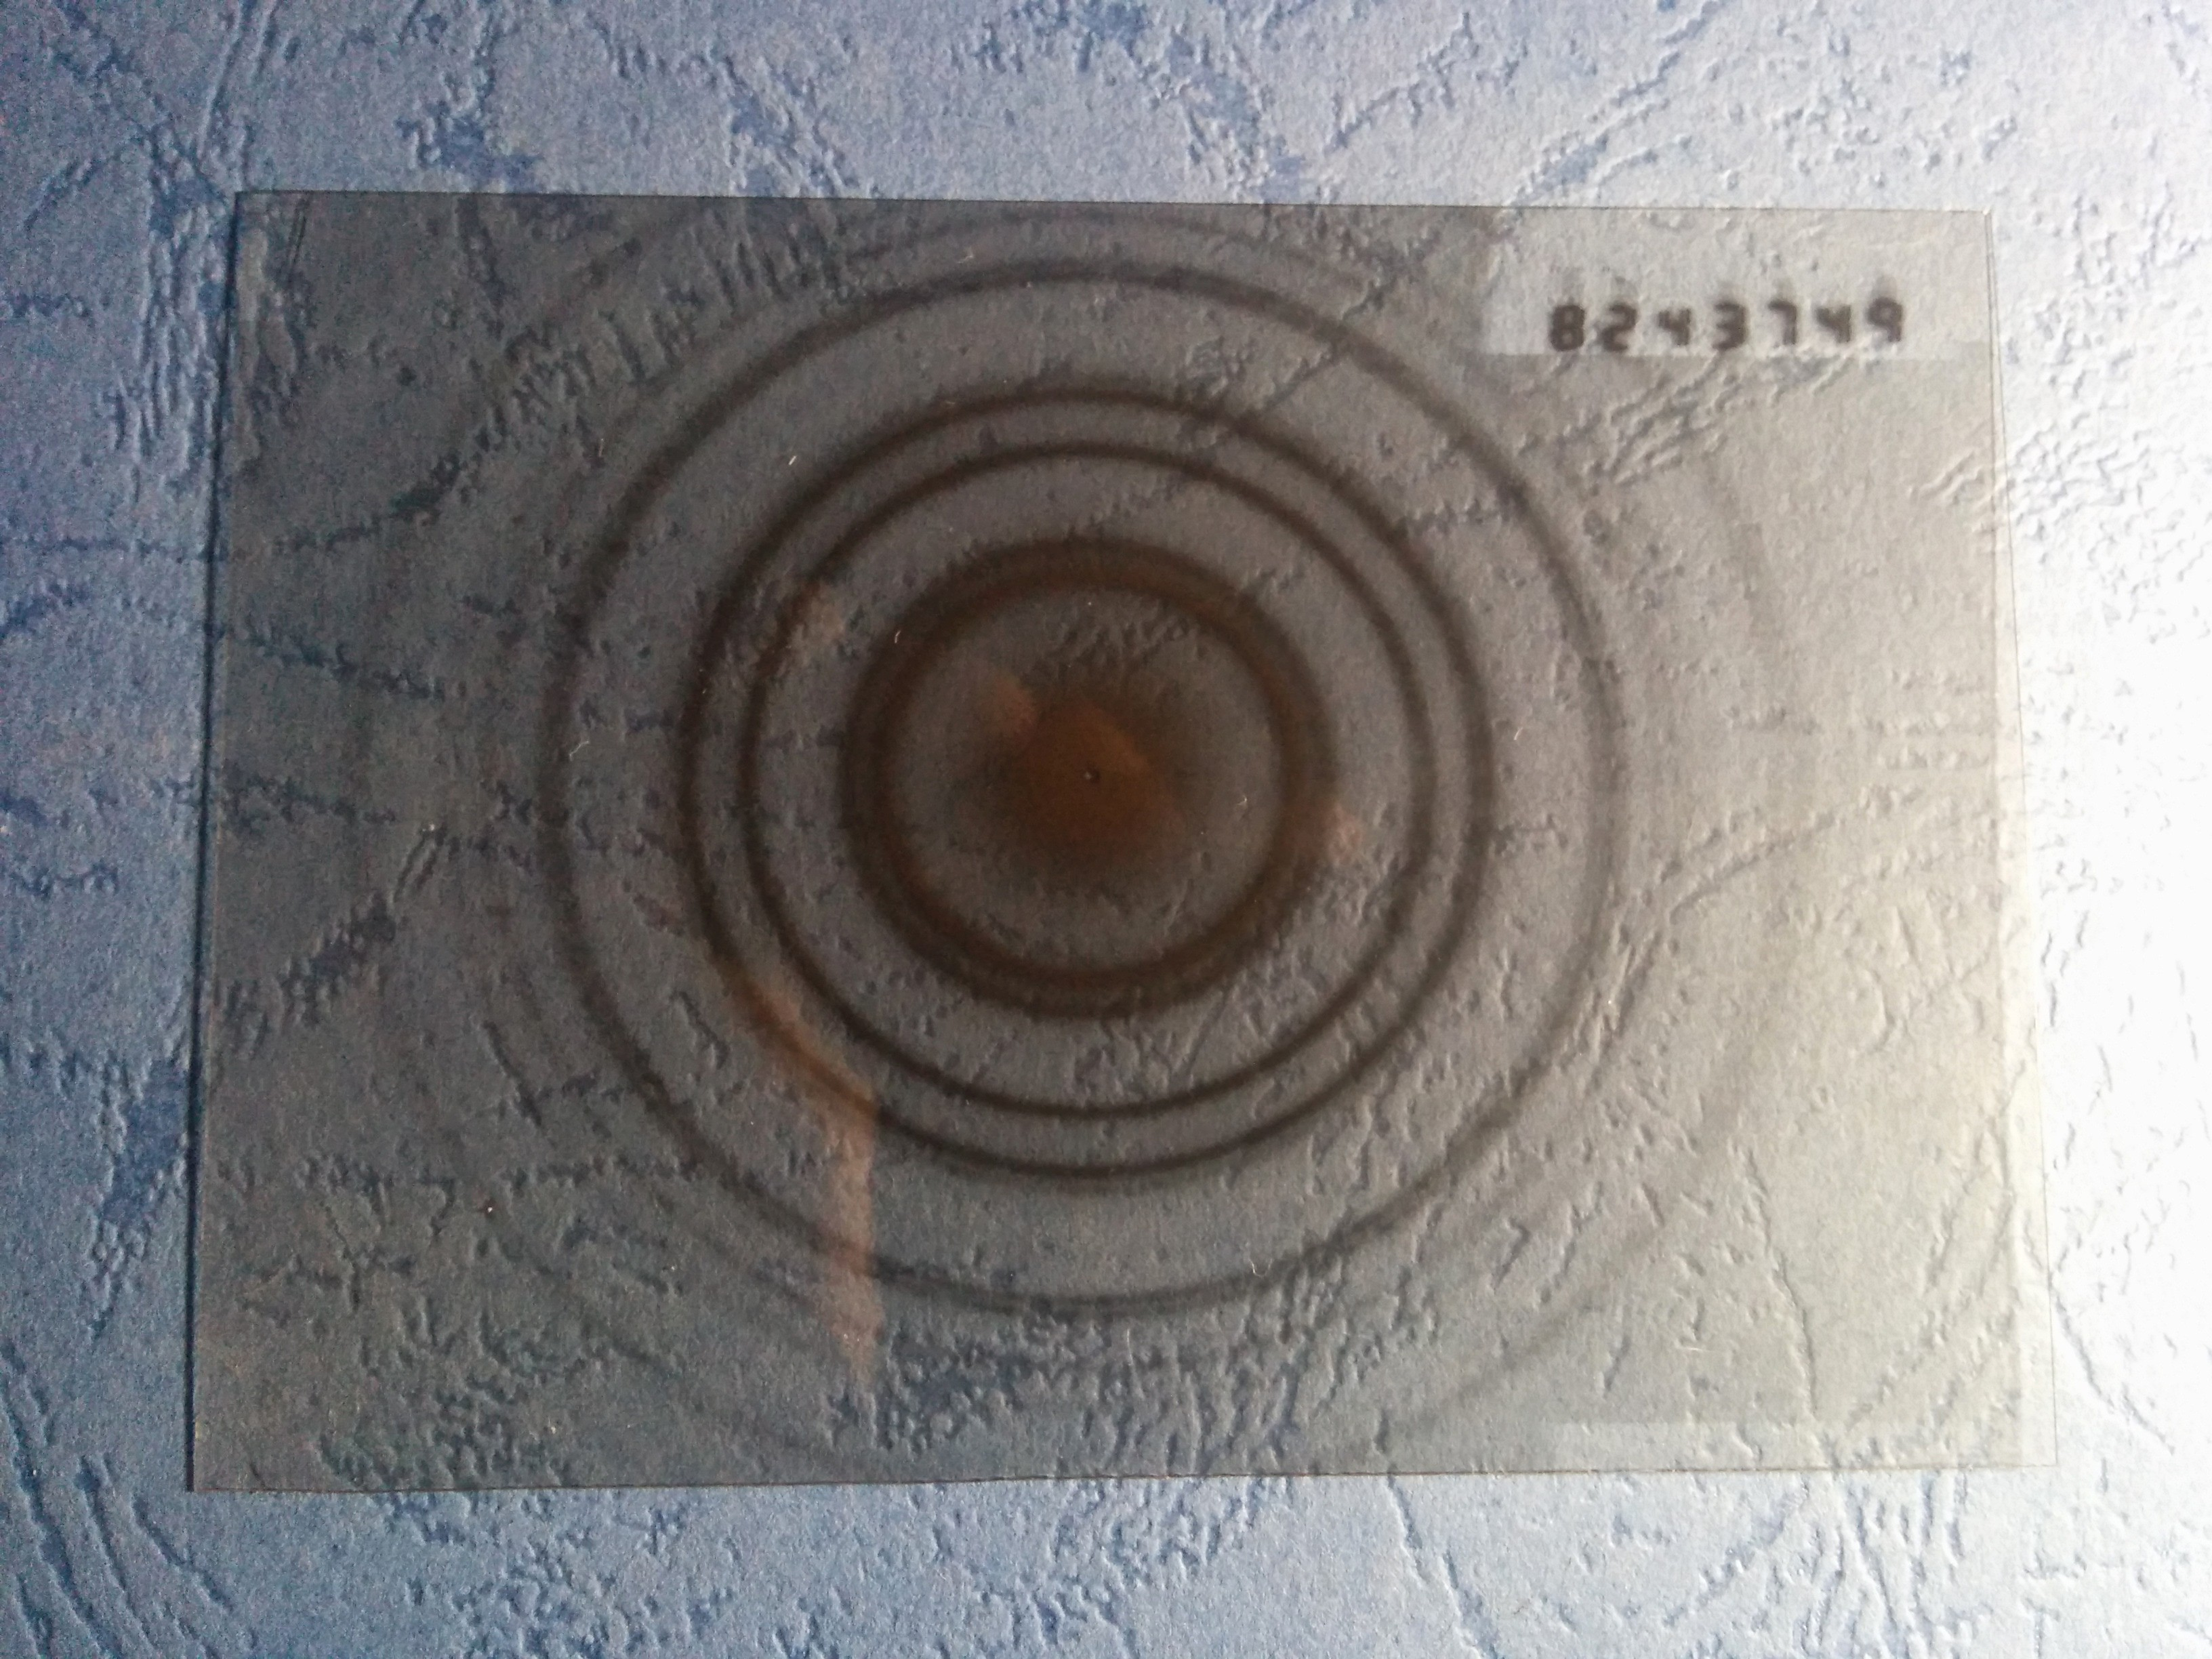
\includegraphics[width=0.3\textwidth]{pic1.png}
		}
		\subfigure{
			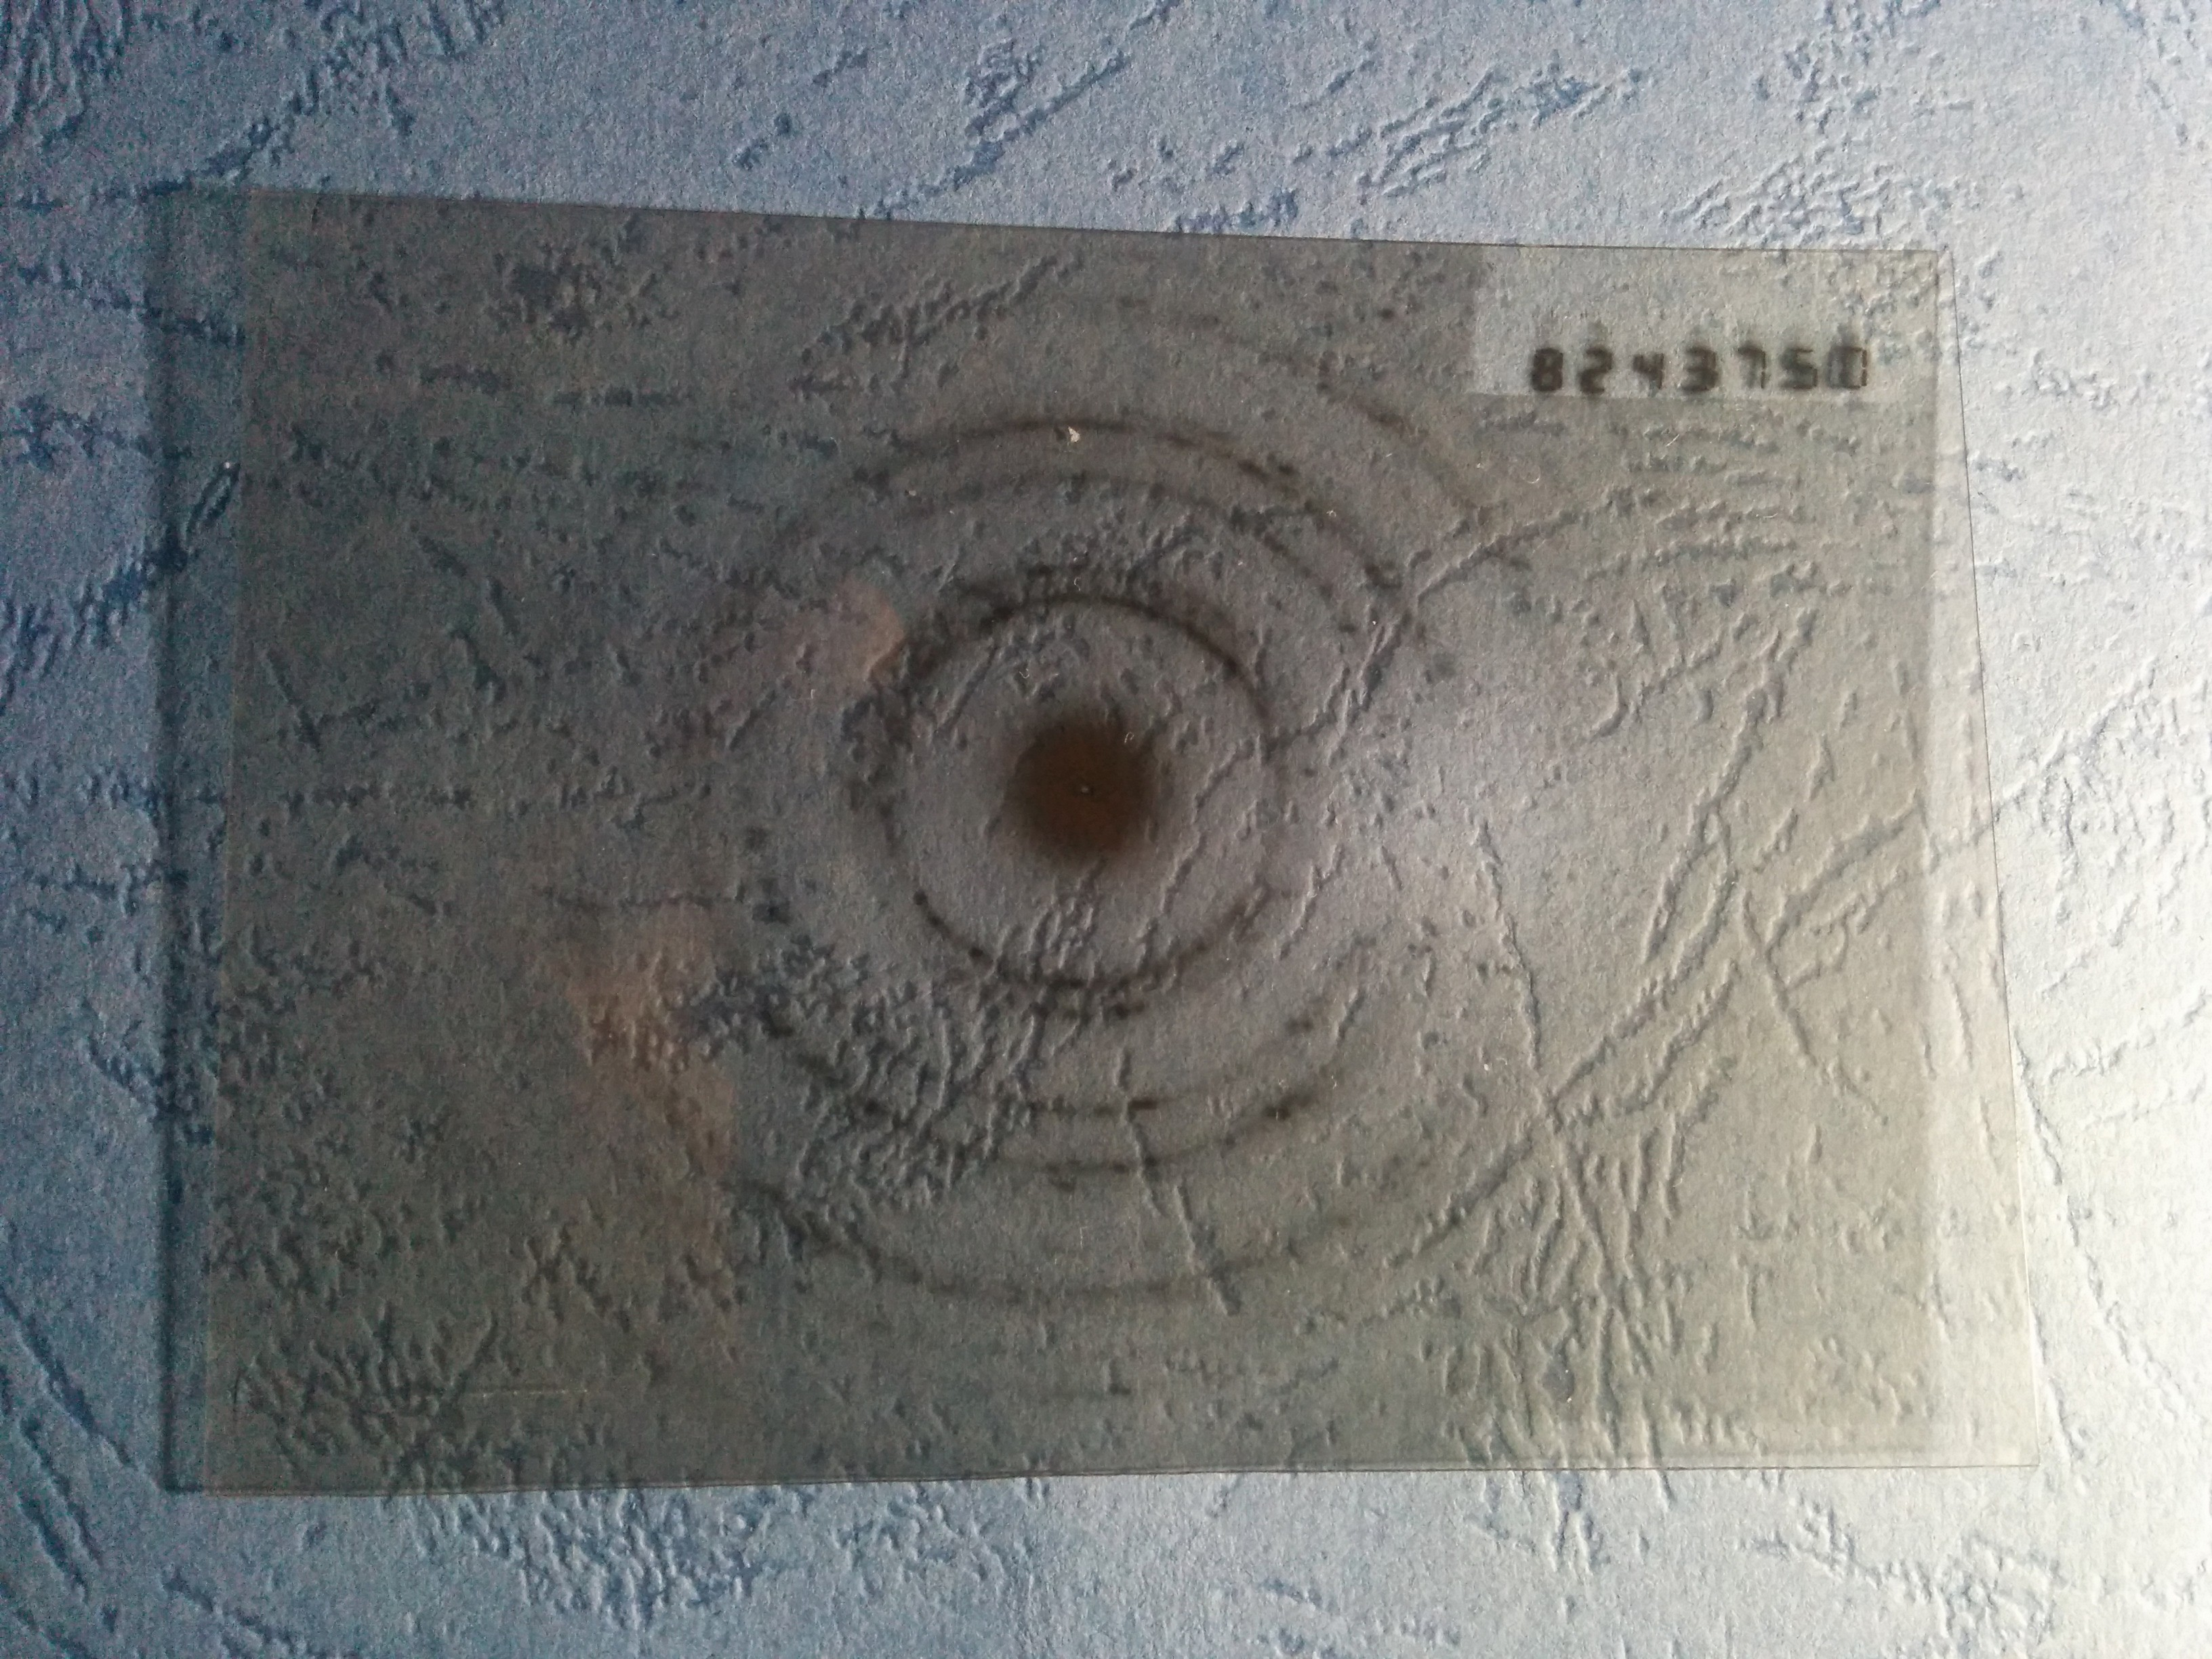
\includegraphics[width=0.3\textwidth]{pic2.png}
		}
		\subfigure{
			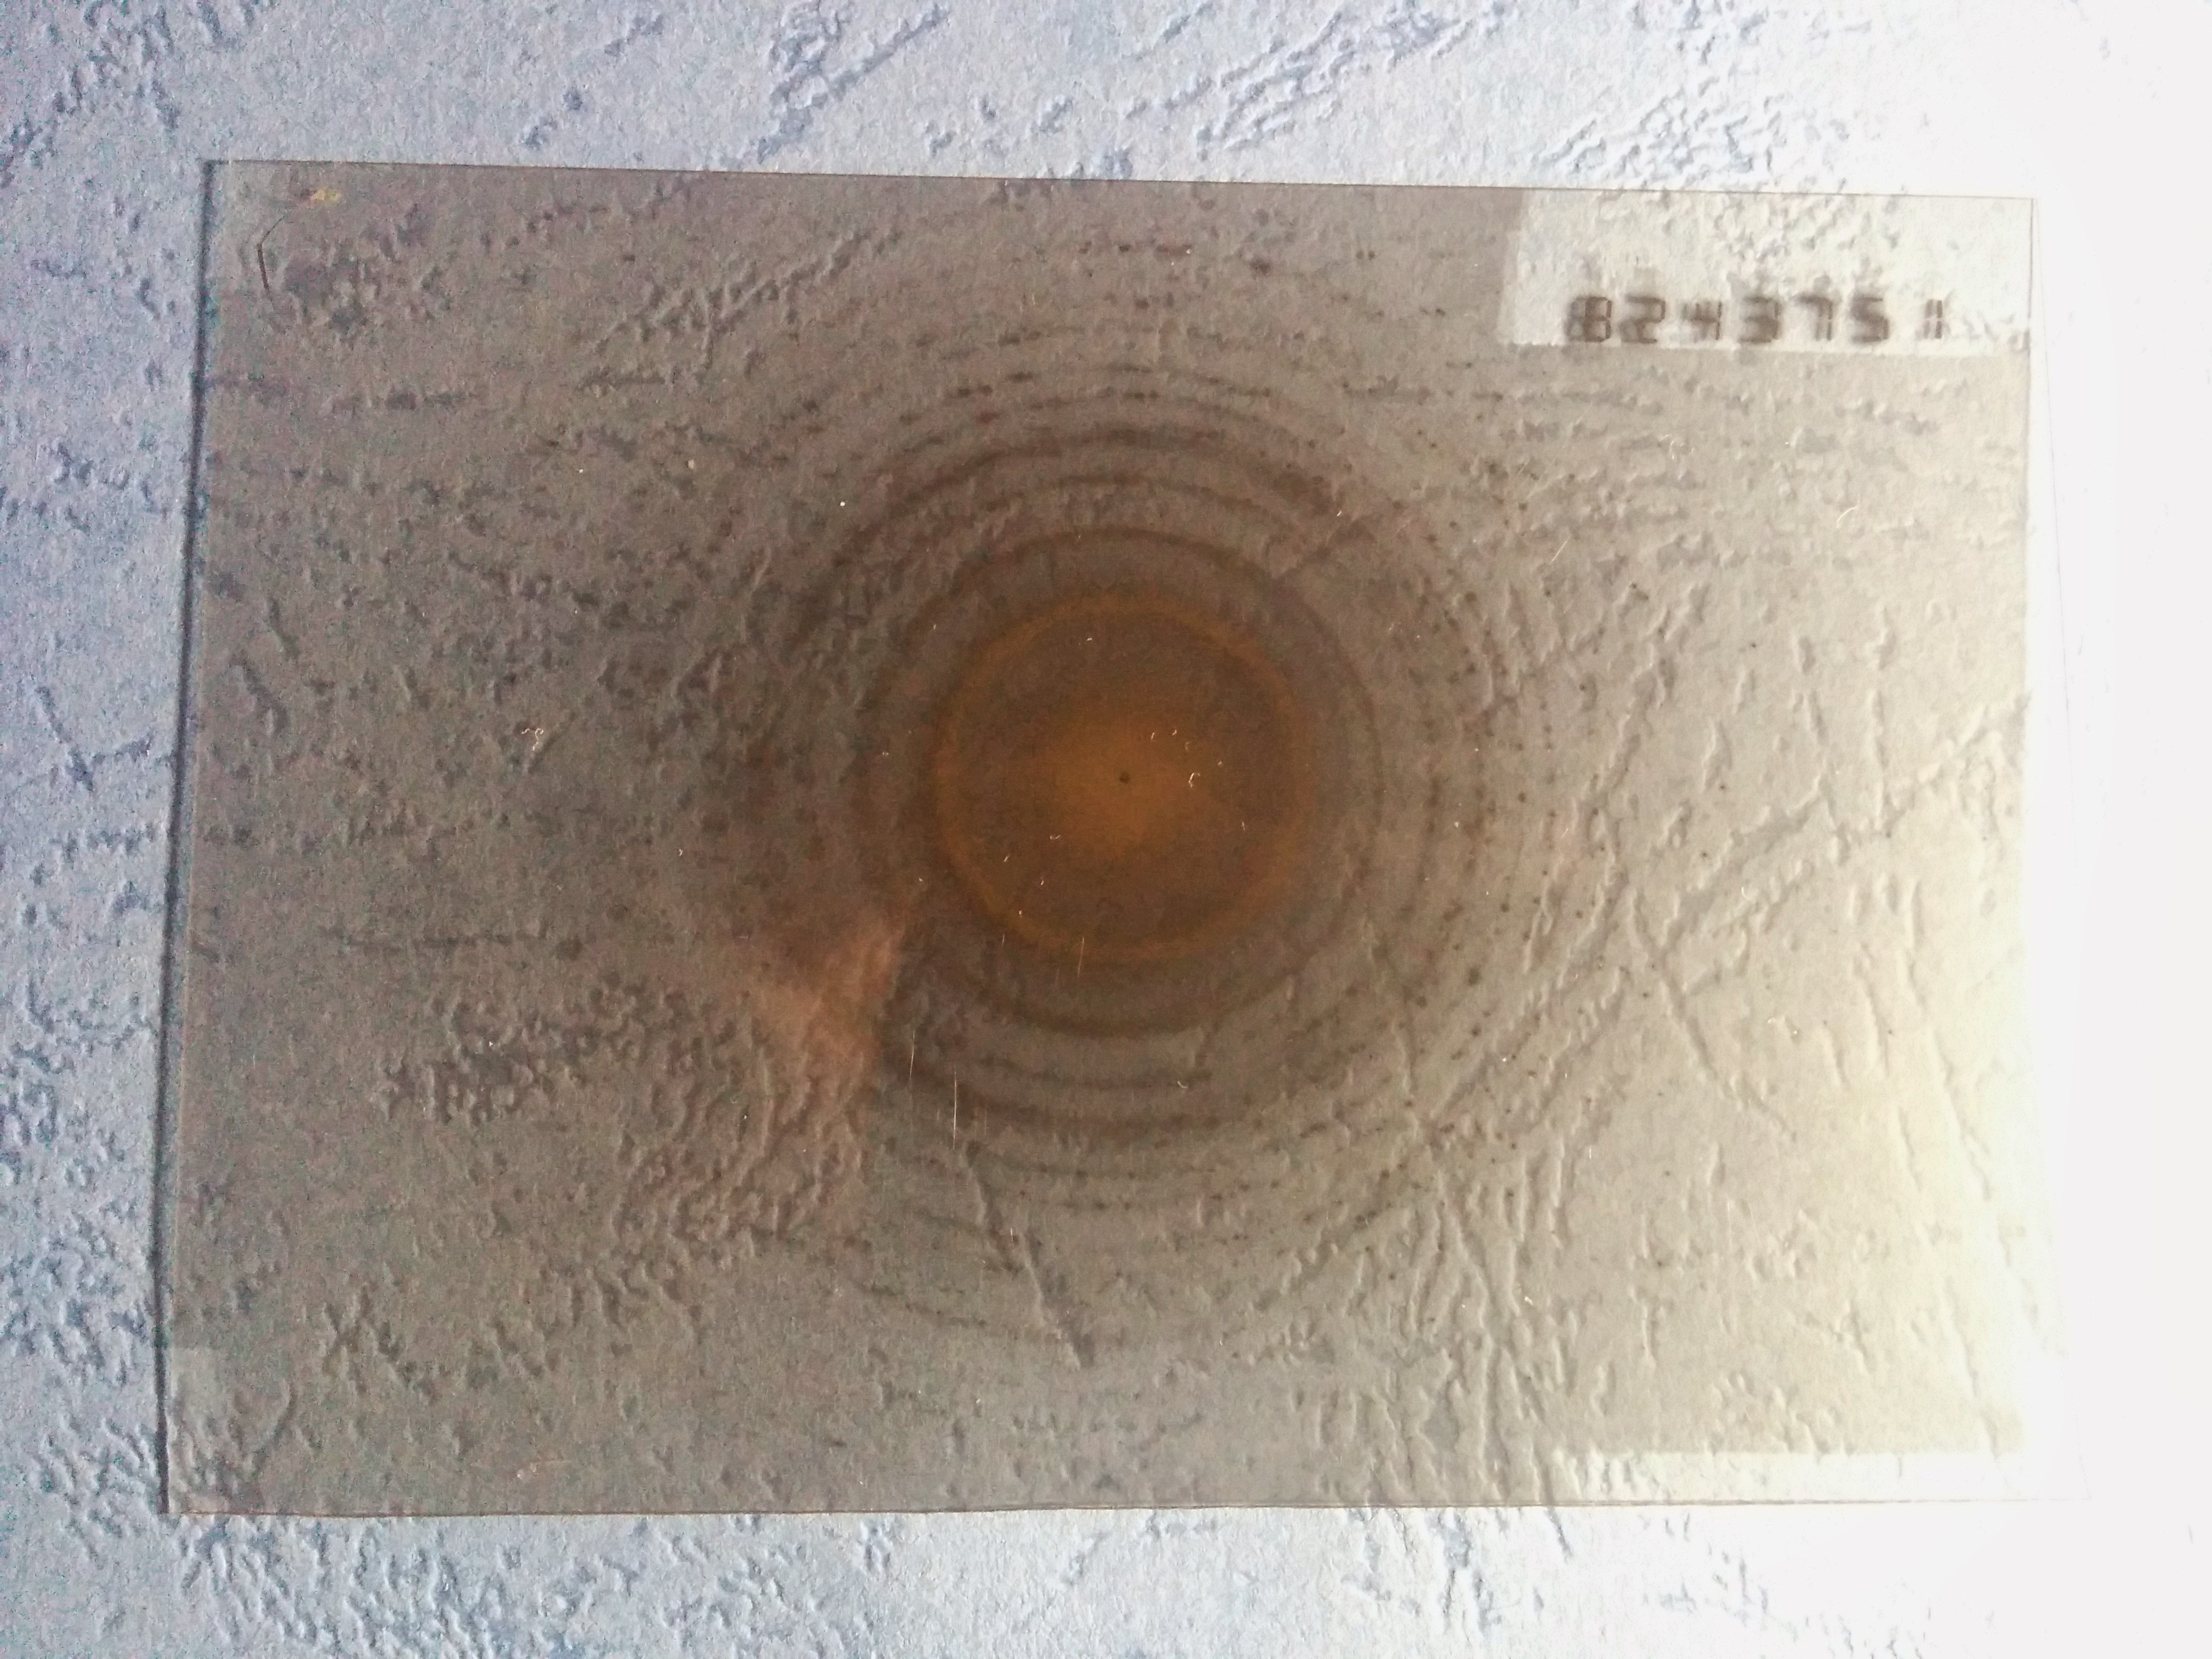
\includegraphics[width=0.3\textwidth]{pic3.png}
		}\\
		\subfigure{
			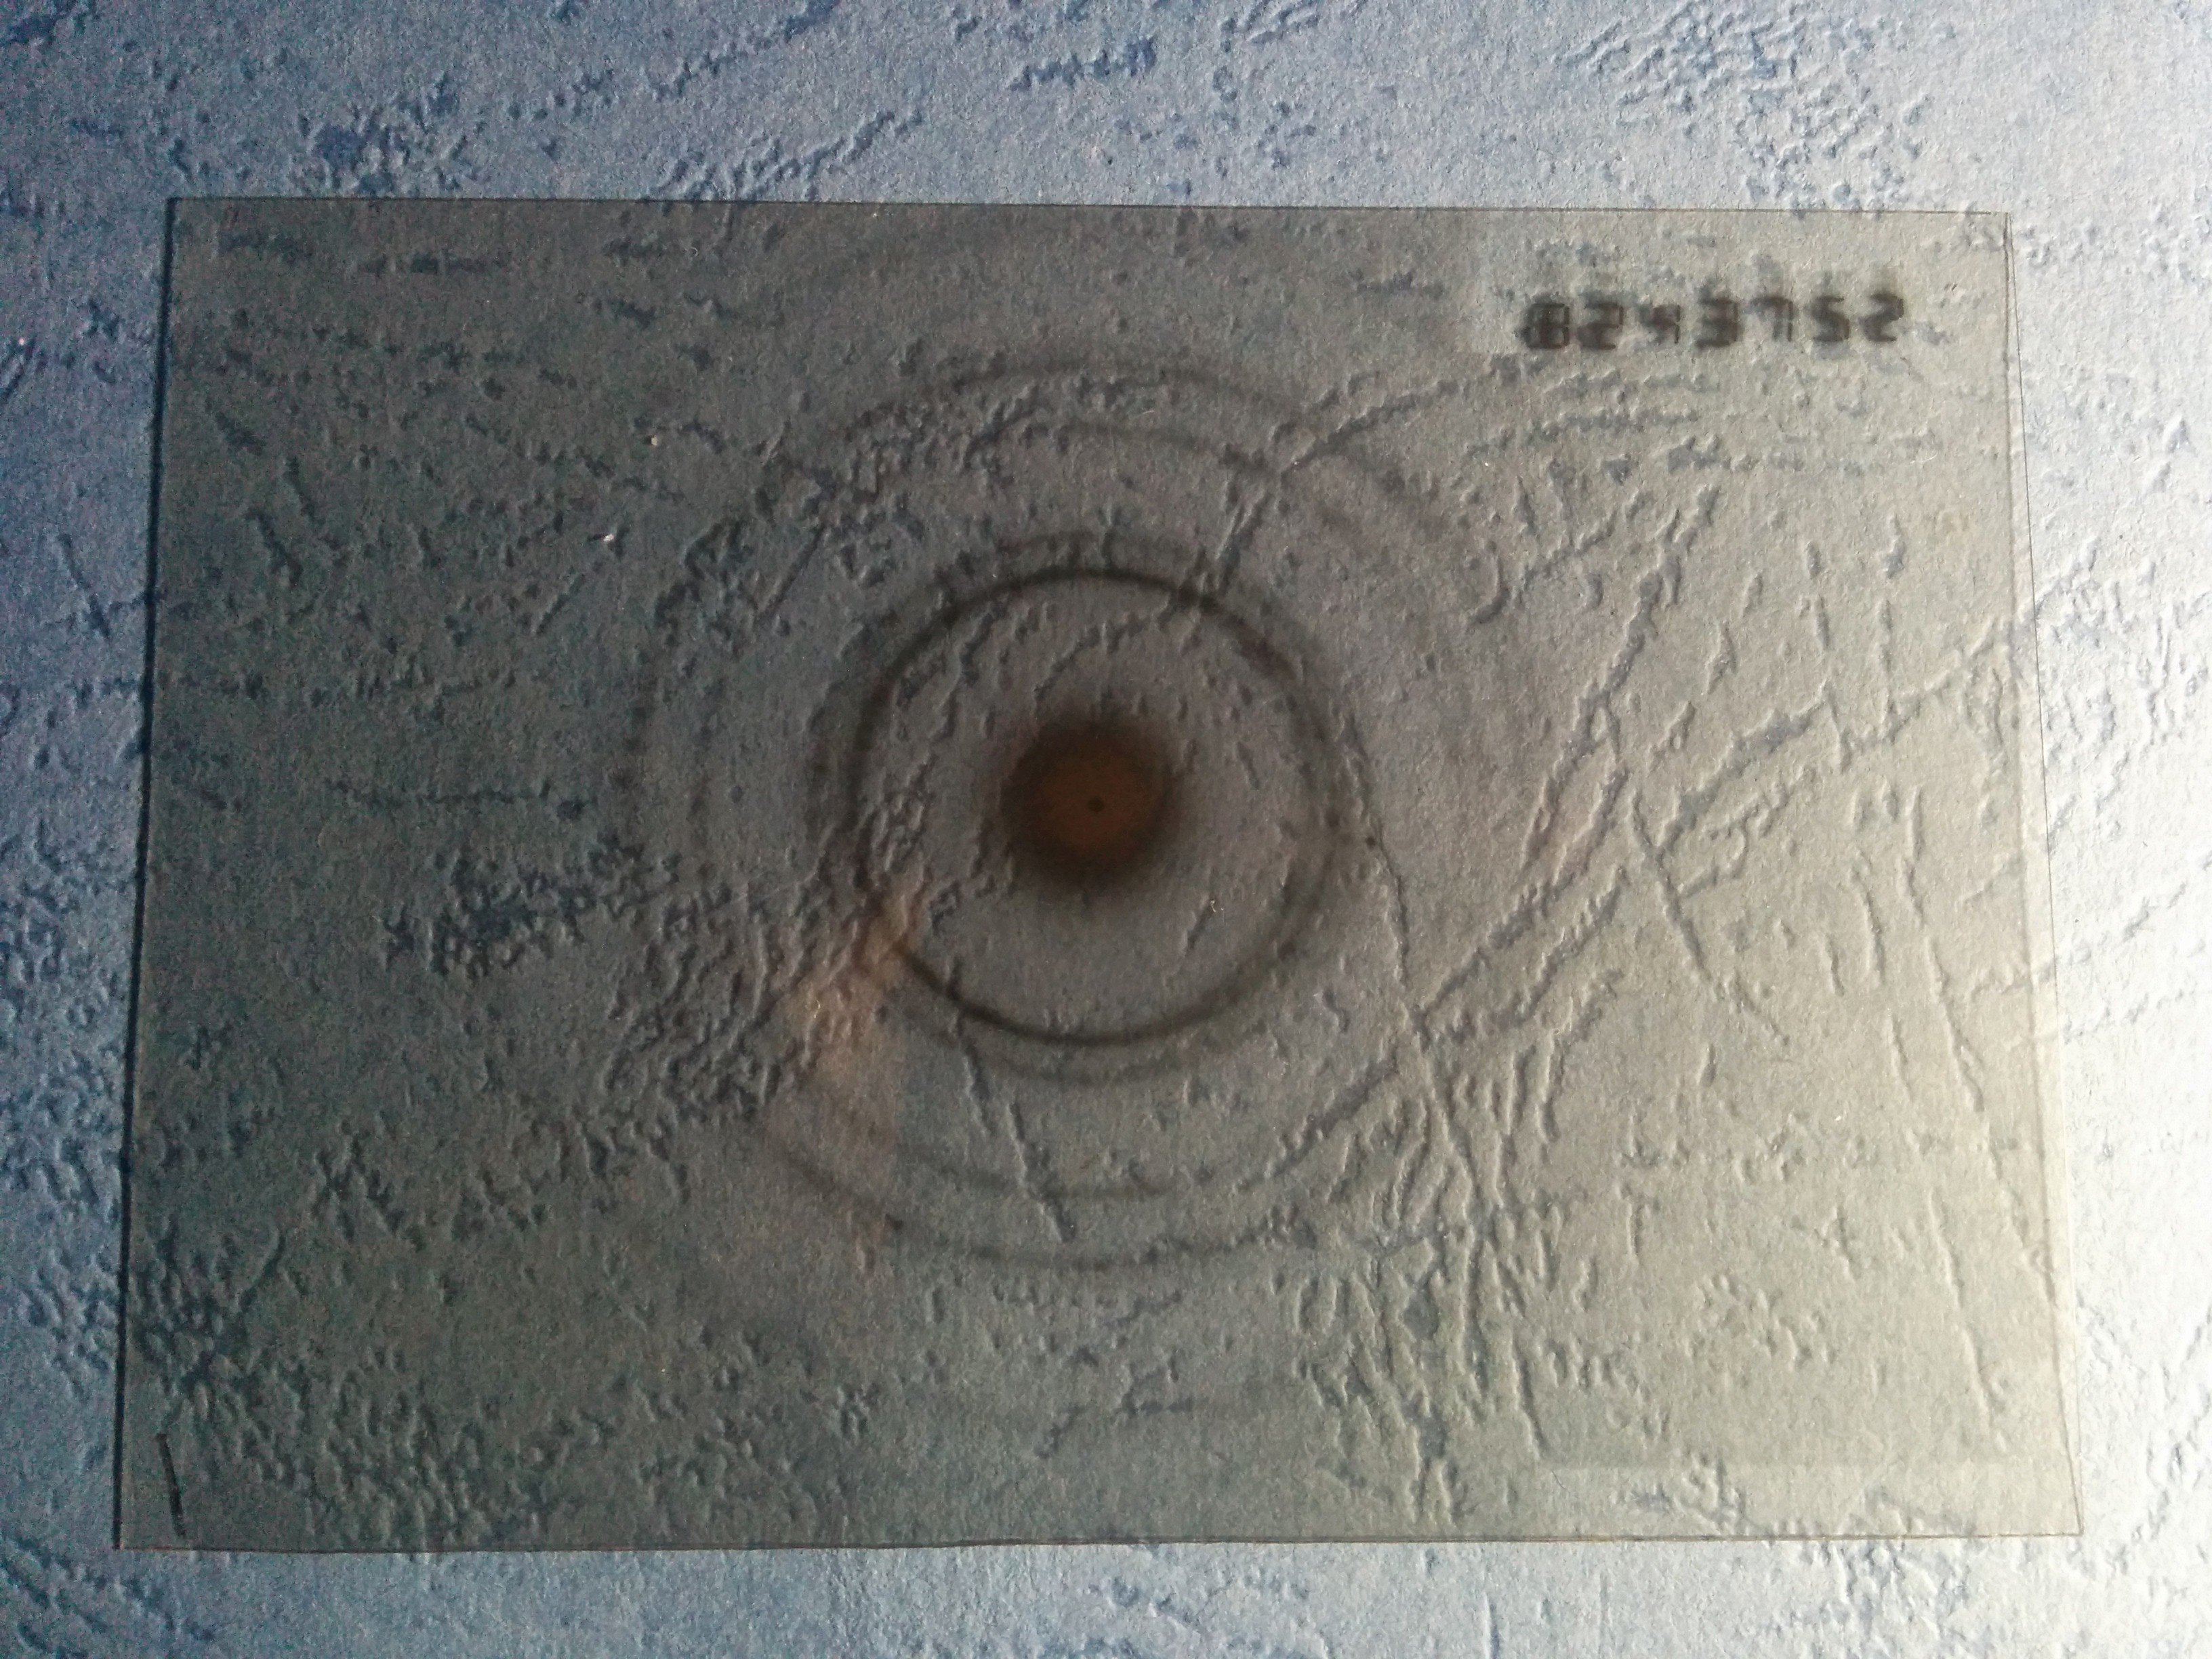
\includegraphics[width=0.3\textwidth]{pic4.png}
		}
		\subfigure{
			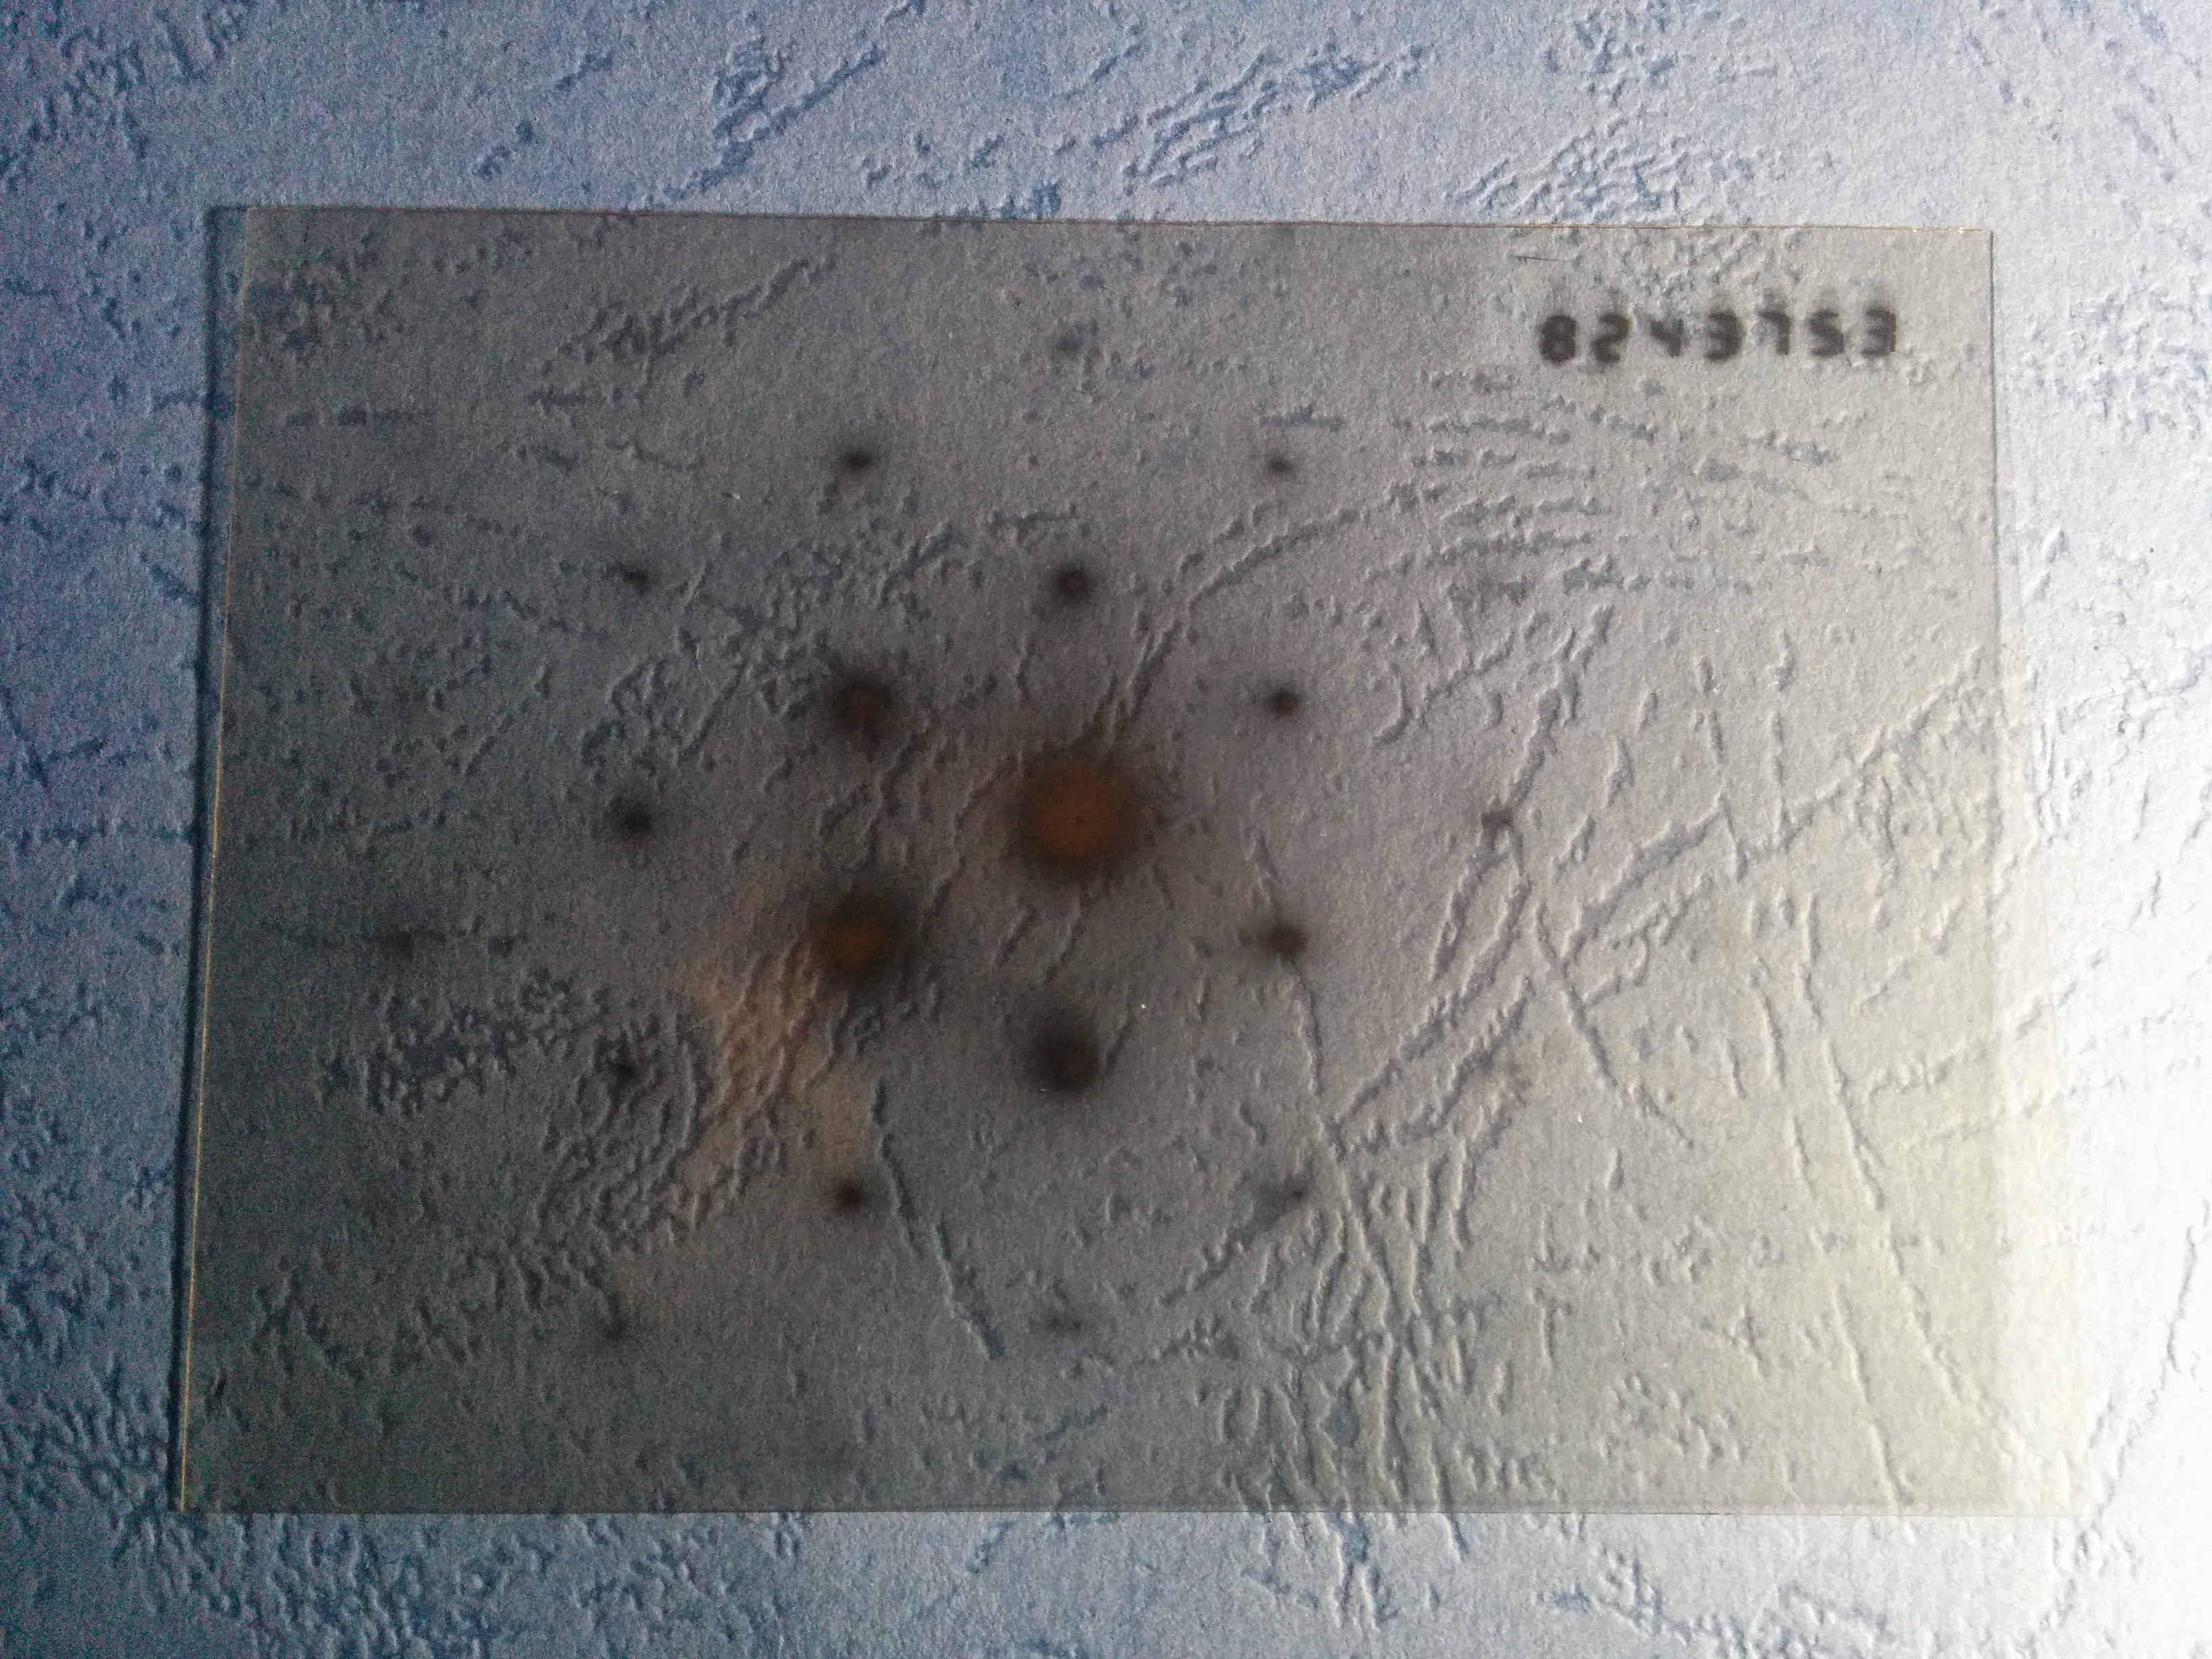
\includegraphics[width=0.3\textwidth]{pic5.png}
		}
		\caption{\label{fig:exp1}电子衍射图样。左上:Au 中上:Ag 右上:Sn 左下:Cu 右下:Si}
	\end{center}
\end{figure}


利用样品Au进行定标。如图所示,样品金的衍射图样呈现为均匀的圆环,可以看出其为多晶体。金的晶格常数$a_0=4.0786\AA$,根据已知的晶格指数和环的关系可以对本次实验进行定标。由关系:
\begin{equation}
	\sin{\theta}=\lambda\sqrt{h^2+k^2+l^2}/2a_0
\end{equation}
可以得到对应的$\sin{\theta}$和直径d之间的关系。假定$\lambda=1.5\AA$,这个值随后会被消除而不会影响到最后的结果。

Au的数据如下,其中直径d的读数误差都为$\frac{\sqrt{3}}{3}=0.06cm$:
\begin{center}
	\begin{table}[h]
		\caption{金衍射图片直径和衍射角之间的关系}
		\begin{tabularx}{10cm}{XXX}
			\hline
			\hline
			$h^2+k^2+l^2$&$\sin{\theta}$&d/cm\\
			\hline
			3&0.318&2.05\\
			4&0.368&2.40\\
			8&0.520&3.40\\
			11&0.610&3.98\\
			12&0.637&4.15\\
			16&0.736&4.80\\
			19&0.802&5.23\\
			20&0.822&5.38\\
			24&0.901&5.90\\
			27&0.956&6.25\\
			\hline
			\hline
		\end{tabularx}
	\end{table}
\end{center}

对其进行拟合做图可以得到如下的图片:

\begin{figure}[h]
	\begin{center}
		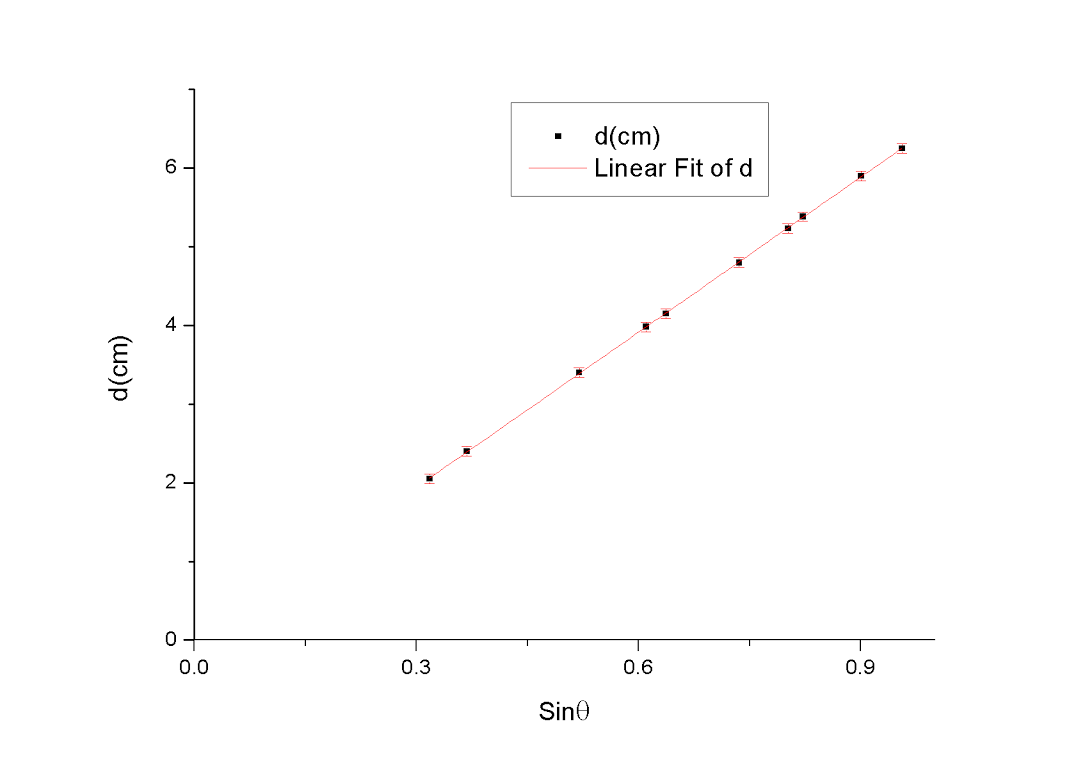
\includegraphics[width=0.8\textwidth]{pic6.png}
		\caption{\label{fig:exp2}Au $\sin{\theta}$与直径d之间的关系}
	\end{center}
\end{figure}
\newpage

拟合得到的斜率为$k=6.57\pm0.01 cm$由此可以定标出其他样品的晶格常数。

接下来研究的是Ag。同样的,银的衍射图样也是圆环状,即为多晶体。根据上文中的斜率可以得到其各个环对应的衍射角度。数据表如下:

\begin{center}
	\begin{table}[h]
		\caption{银衍射图片直径和衍射角之间的关系表}
		\begin{tabularx}{10cm}{XX}
			\hline
			\hline
			d/cm&$\sin{\theta}$\\
			\hline
			2.06&0.314\\
			2.38&0.362\\
			3.35&0.510\\
			3.90&0.594\\
			4.10&0.624\\
			\hline
			\hline
		\end{tabularx}
	\end{table}
\end{center}
对其进行指标化,如下图所示:
\begin{figure}[h]
	\begin{center}
		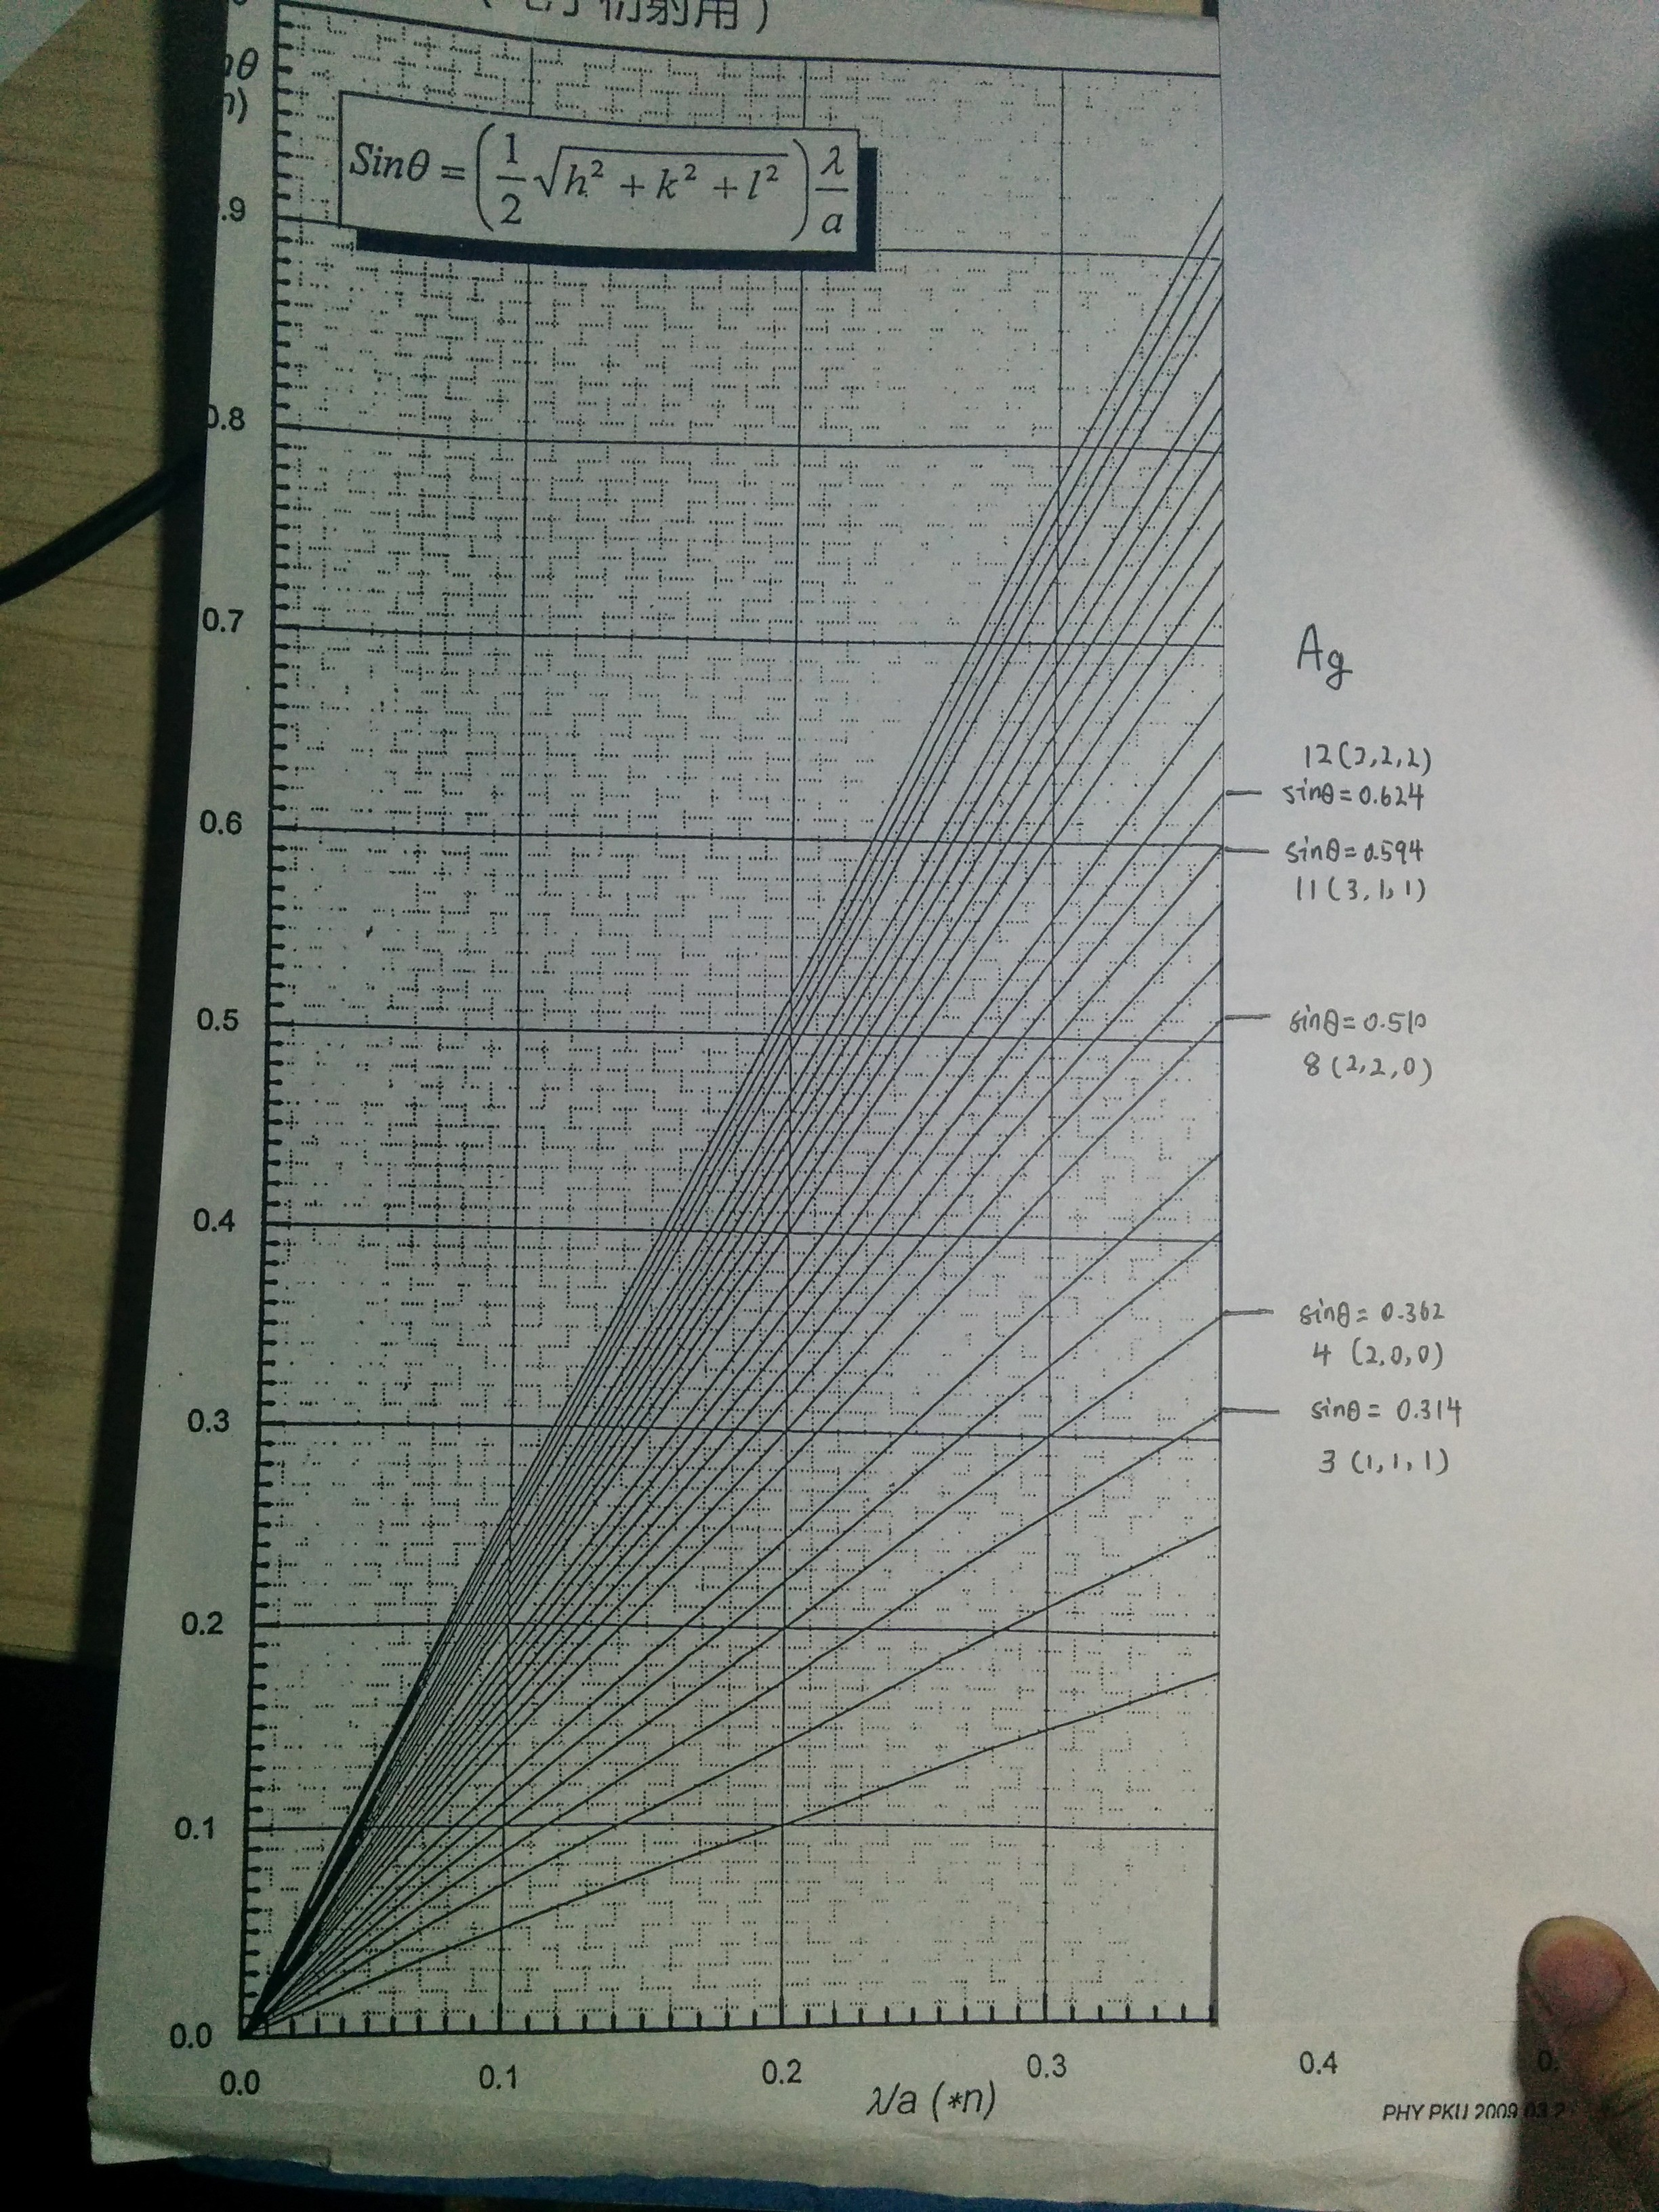
\includegraphics[width=0.55\textwidth]{Ag.png}
		\caption{\label{fig:exp2}Ag 指标化示意图}
	\end{center}
\end{figure}

如图所示可以得到银的晶格常数满足:
\begin{equation}
	\frac{\lambda}{a_0}=0.362
\end{equation}
从而得到Ag的晶格常数为 $a_0=4.1\AA$,同时也得到了其5条晶面指数组合分别为(1,1,1),(2,0,0),(2,2,0),(3,1,1),(2,2,2)。可知Ag为面心立方。

然后是Sn。锡的衍射图样也是圆环状,即为多晶体。根据斜率可以得到其各个环对应的衍射角度。数据表如下:

\begin{center}
	\begin{table}[h]
		\caption{锡衍射图片直径和衍射角之间的关系表}
		\begin{tabularx}{10cm}{XX}
			\hline
			\hline
			d/cm&$\sin{\theta}$\\
			\hline
			1.68&0.256\\
			1.81&0.275\\
			2.45&0.373\\
			2.98&0.454\\
			3.34&0.508\\
			3.42&0.521\\
			3.54&0.539\\
			3.84&0.584\\
			\hline
			\hline
		\end{tabularx}
	\end{table}
\end{center}
对其进行指标化,如下图所示:
\newpage
\begin{figure}[h]
	\begin{center}
		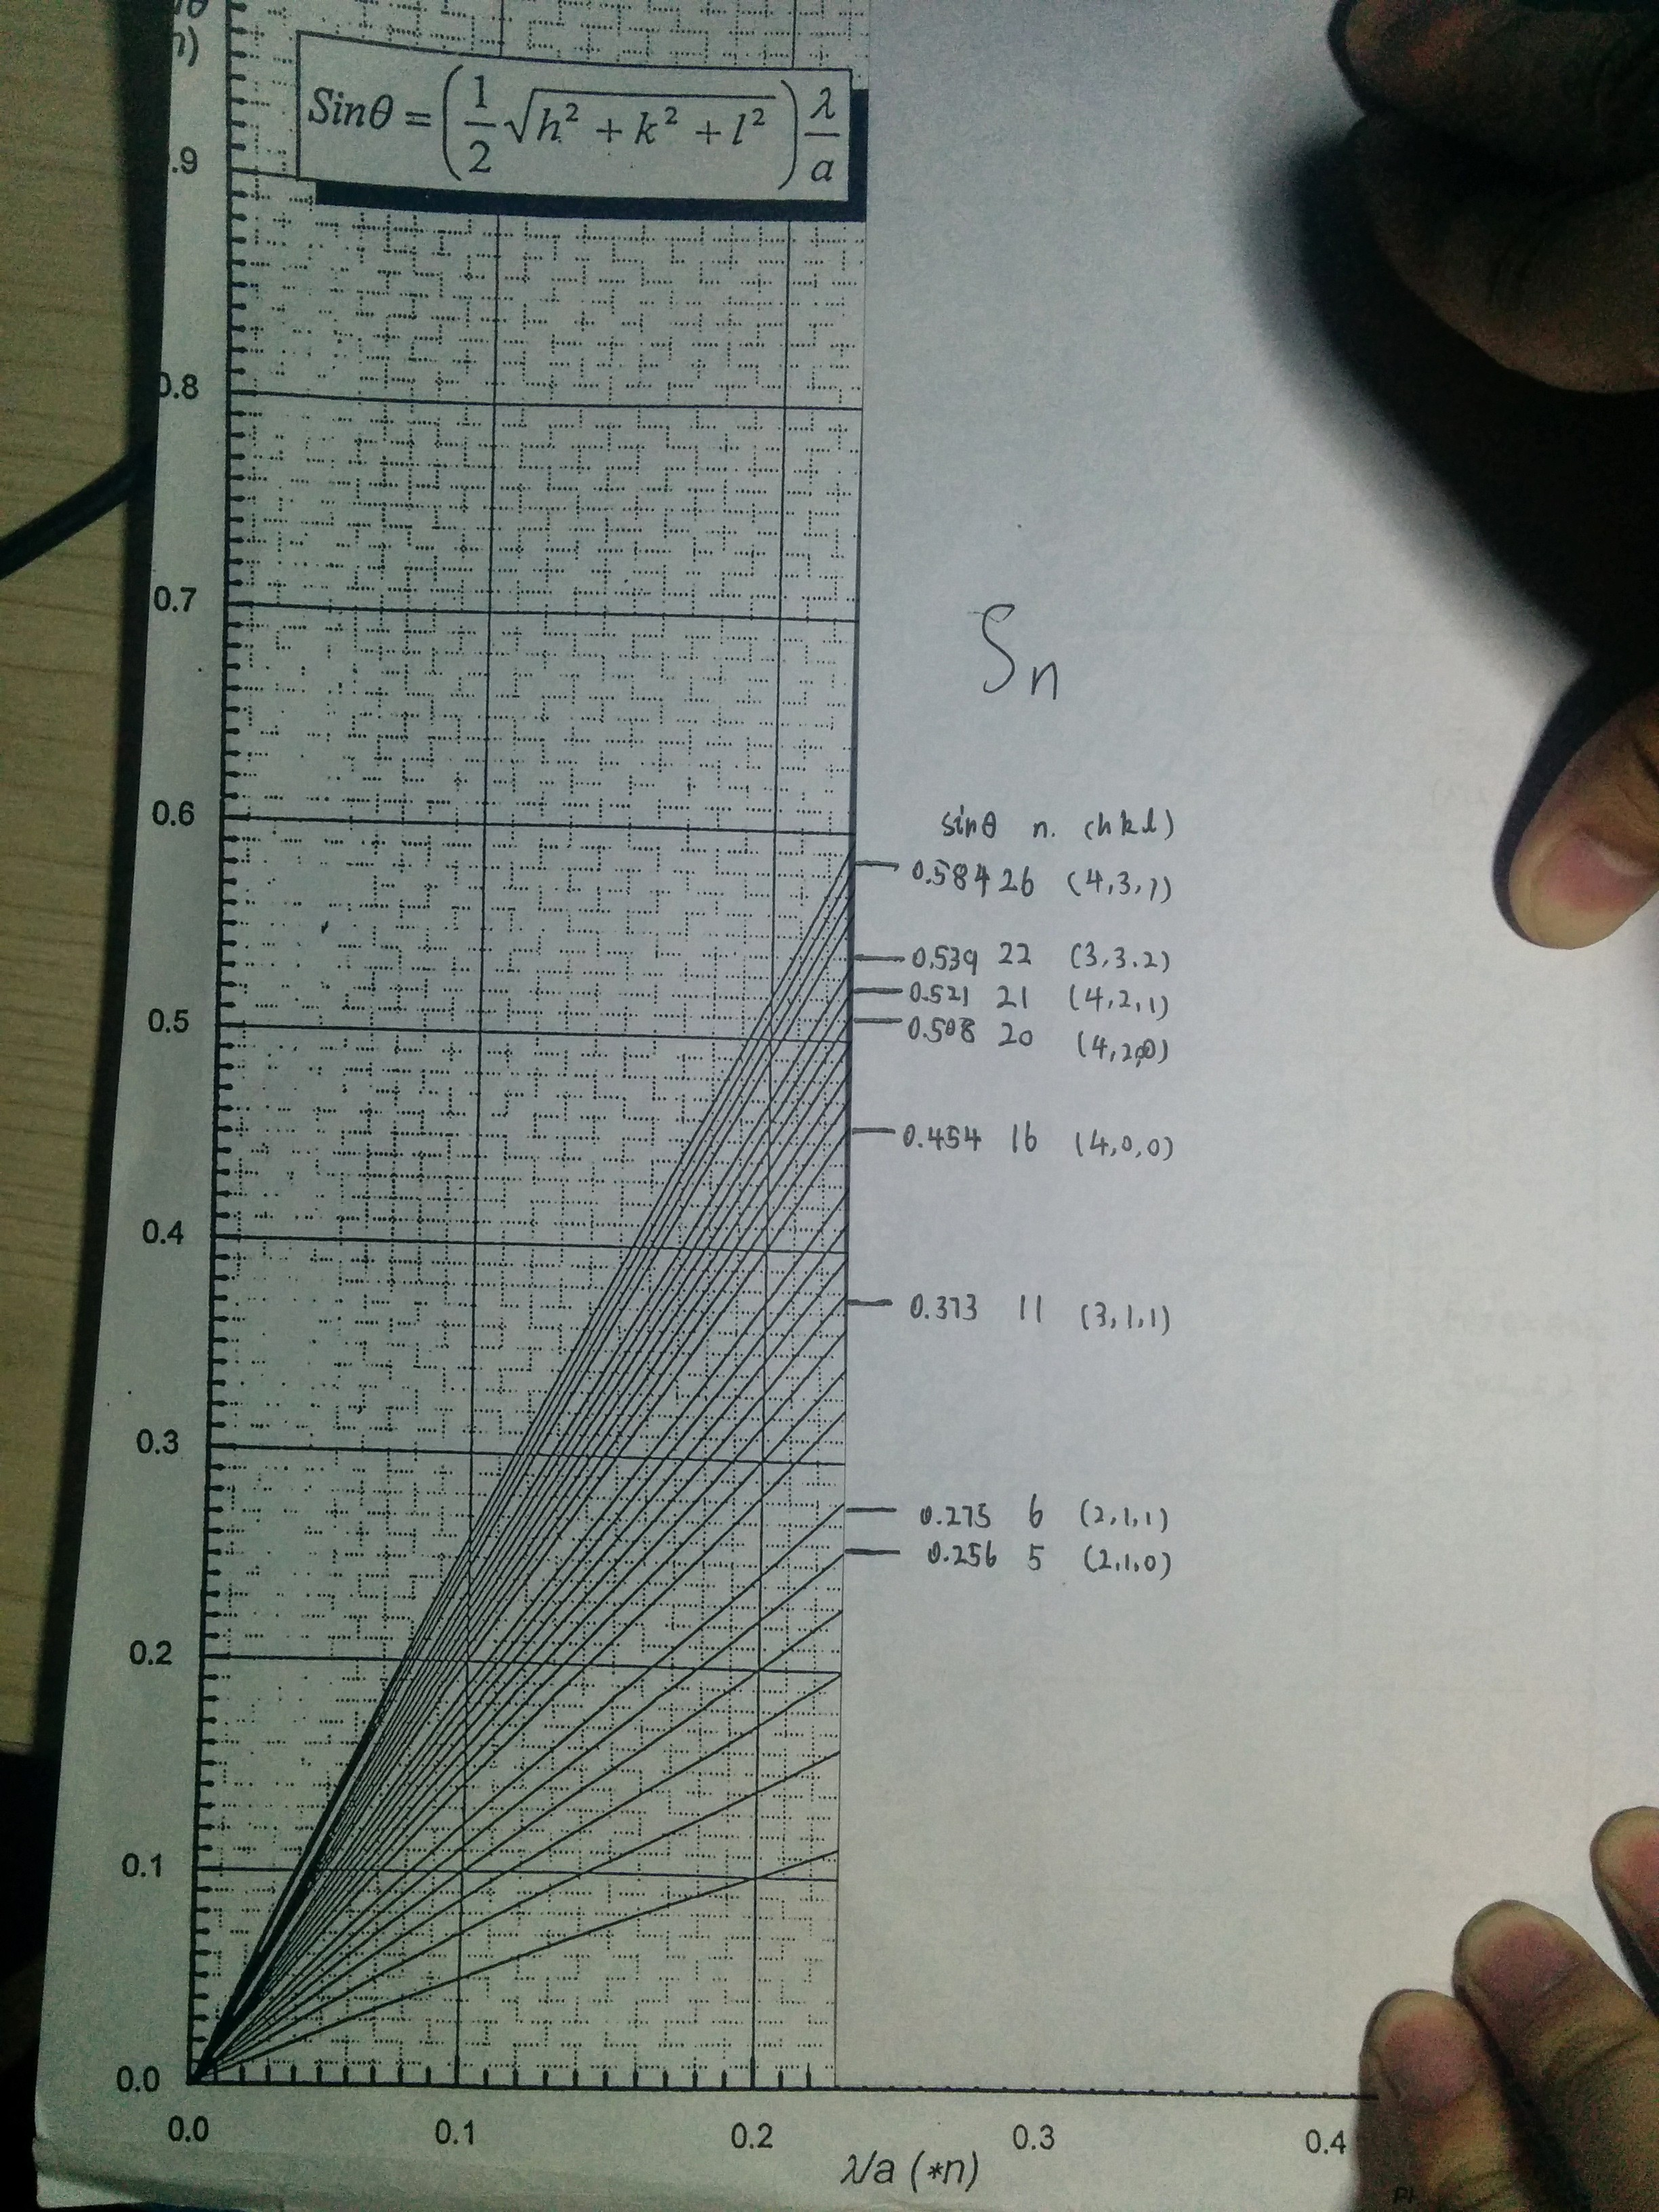
\includegraphics[width=0.55\textwidth]{Sn.png}
		\caption{\label{fig:exp2}Sn 指标化示意图}
	\end{center}
\end{figure}

如图所示可以得到锡的晶格常数满足:
\begin{equation}
	\frac{\lambda}{a_0}=0.228
\end{equation}
从而得到Sn的晶格常数为 $a_0=6.5\AA$,同时也得到了其晶面指数组合分别为(2,1,0),(2,1,1),(3,1,1),(4,0,0),(4,2,0),(4,2,1),(3,3,2),(4,3,1)。可见Sn不是一个简单的多晶,其晶胞内的组成各位复杂,是一个复式晶格,并不是简单的面心立方或者体心立方。\cite{guti}。

对于Cu而言。铜的衍射图样也是圆环状,是多晶体。计算可得到其各个环对应的衍射角度。数据表如下:

\begin{center}
	\begin{table}[h]
		\caption{铜衍射图片直径和衍射角之间的关系表}
		\begin{tabularx}{10cm}{XX}
			\hline
			\hline
			d/cm&$\sin{\theta}$\\
			\hline
			2.28&0.347\\
			2.65&0.403\\
			3.75&0.570\\
			4.41&0.671\\
			5.73&0.872\\
			\hline
			\hline
		\end{tabularx}
	\end{table}
\end{center}
\newpage
对其进行指标化,如下图所示:
\begin{figure}[h]
	\begin{center}
		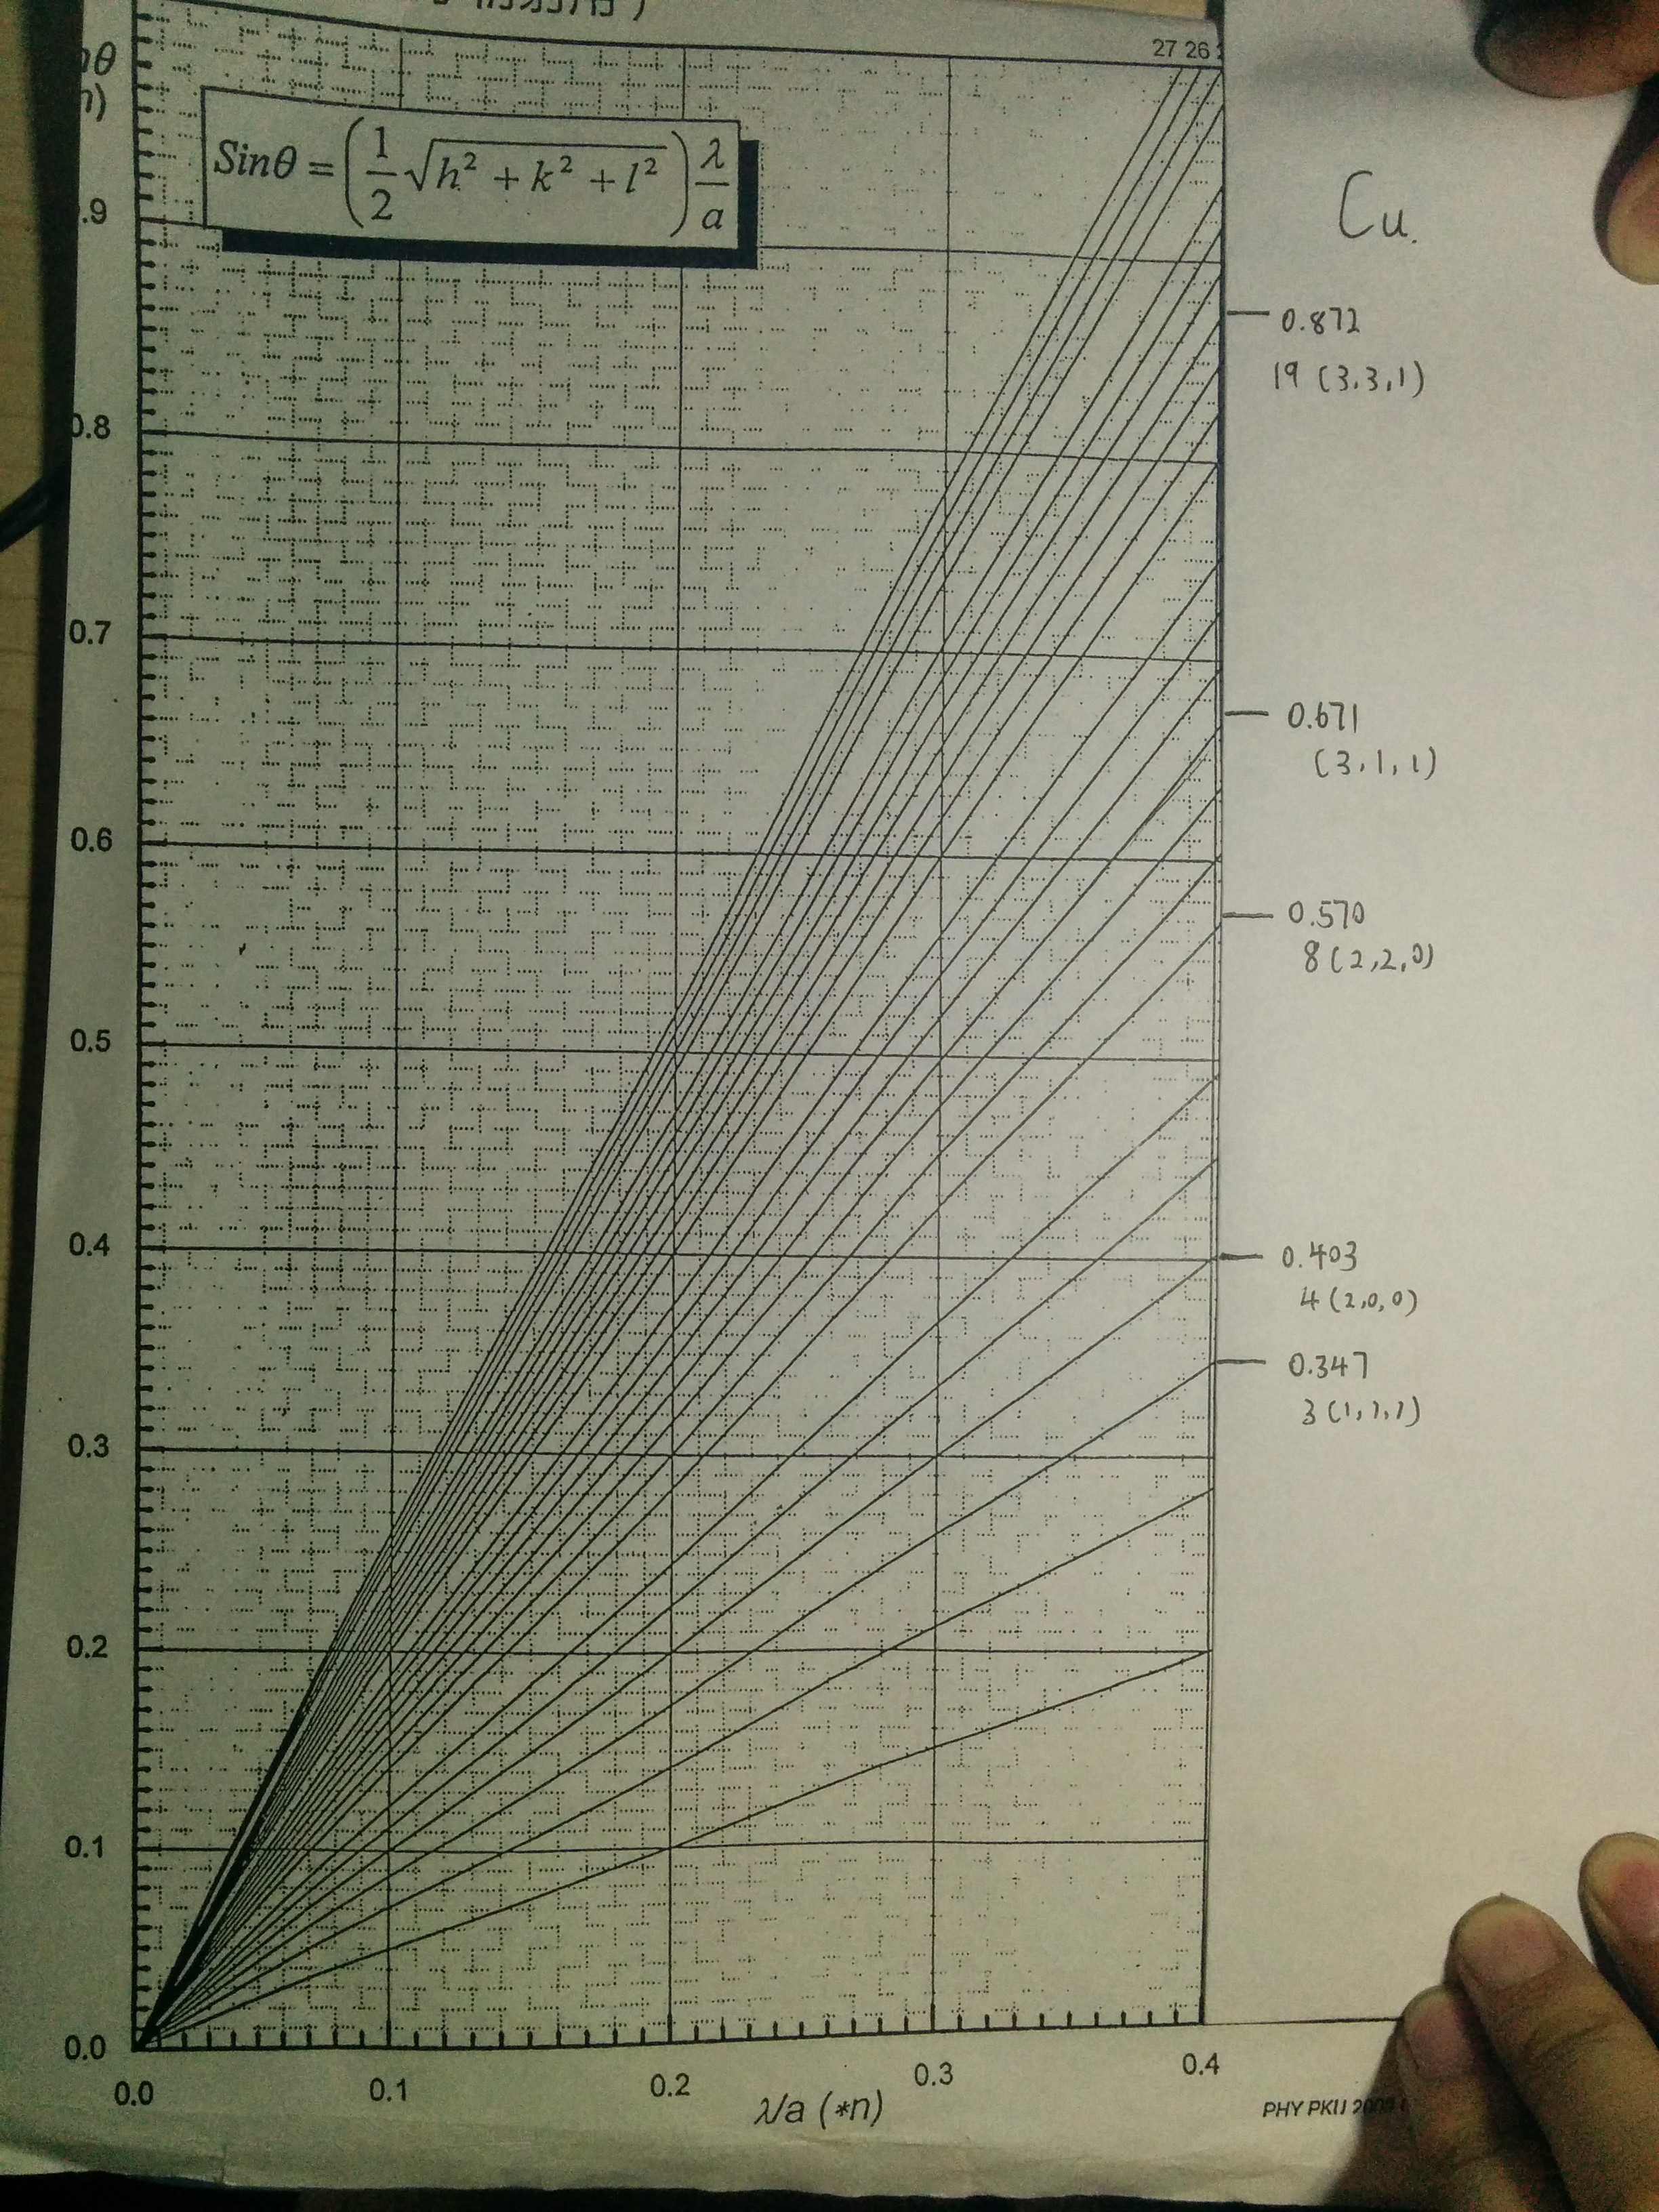
\includegraphics[width=0.55\textwidth]{Cu.png}
		\caption{\label{fig:exp2}Cu 指标化示意图}
	\end{center}
\end{figure}

如图所示可以得到铜的晶格常数满足:
\begin{equation}
	\frac{\lambda}{a_0}=0.41
\end{equation}
从而得到铜的晶格常数为 $a_0=3.6\AA$,同时也得到了其5条晶面指数组合分别为(1,1,1),(2,0,0),(2,2,0),(3,1,1),(3,3,1)。可知铜为面心立方。

最后是硅。同样的,硅的衍射图样成点状分布,所以说硅为单晶体。斑点围绕中心成周期分布,都在一定的圆环上,所以可以测量中心对称两点的衍射距离以得到晶格常数。数据表如下:
\begin{center}
	\begin{table}[h]
		\caption{硅衍射图片直径和衍射角之间的关系表}
		\begin{tabularx}{10cm}{XX}
			\hline
			\hline
			d/cm&$\sin{\theta}$\\
			\hline
			2.46&0.374\\
			4.24&0.645\\
			4.88&0.743\\
			\hline
			\hline
		\end{tabularx}
	\end{table}
\end{center}
对其进行指标化,如下图所示:
\begin{figure}[h]
	\begin{center}
	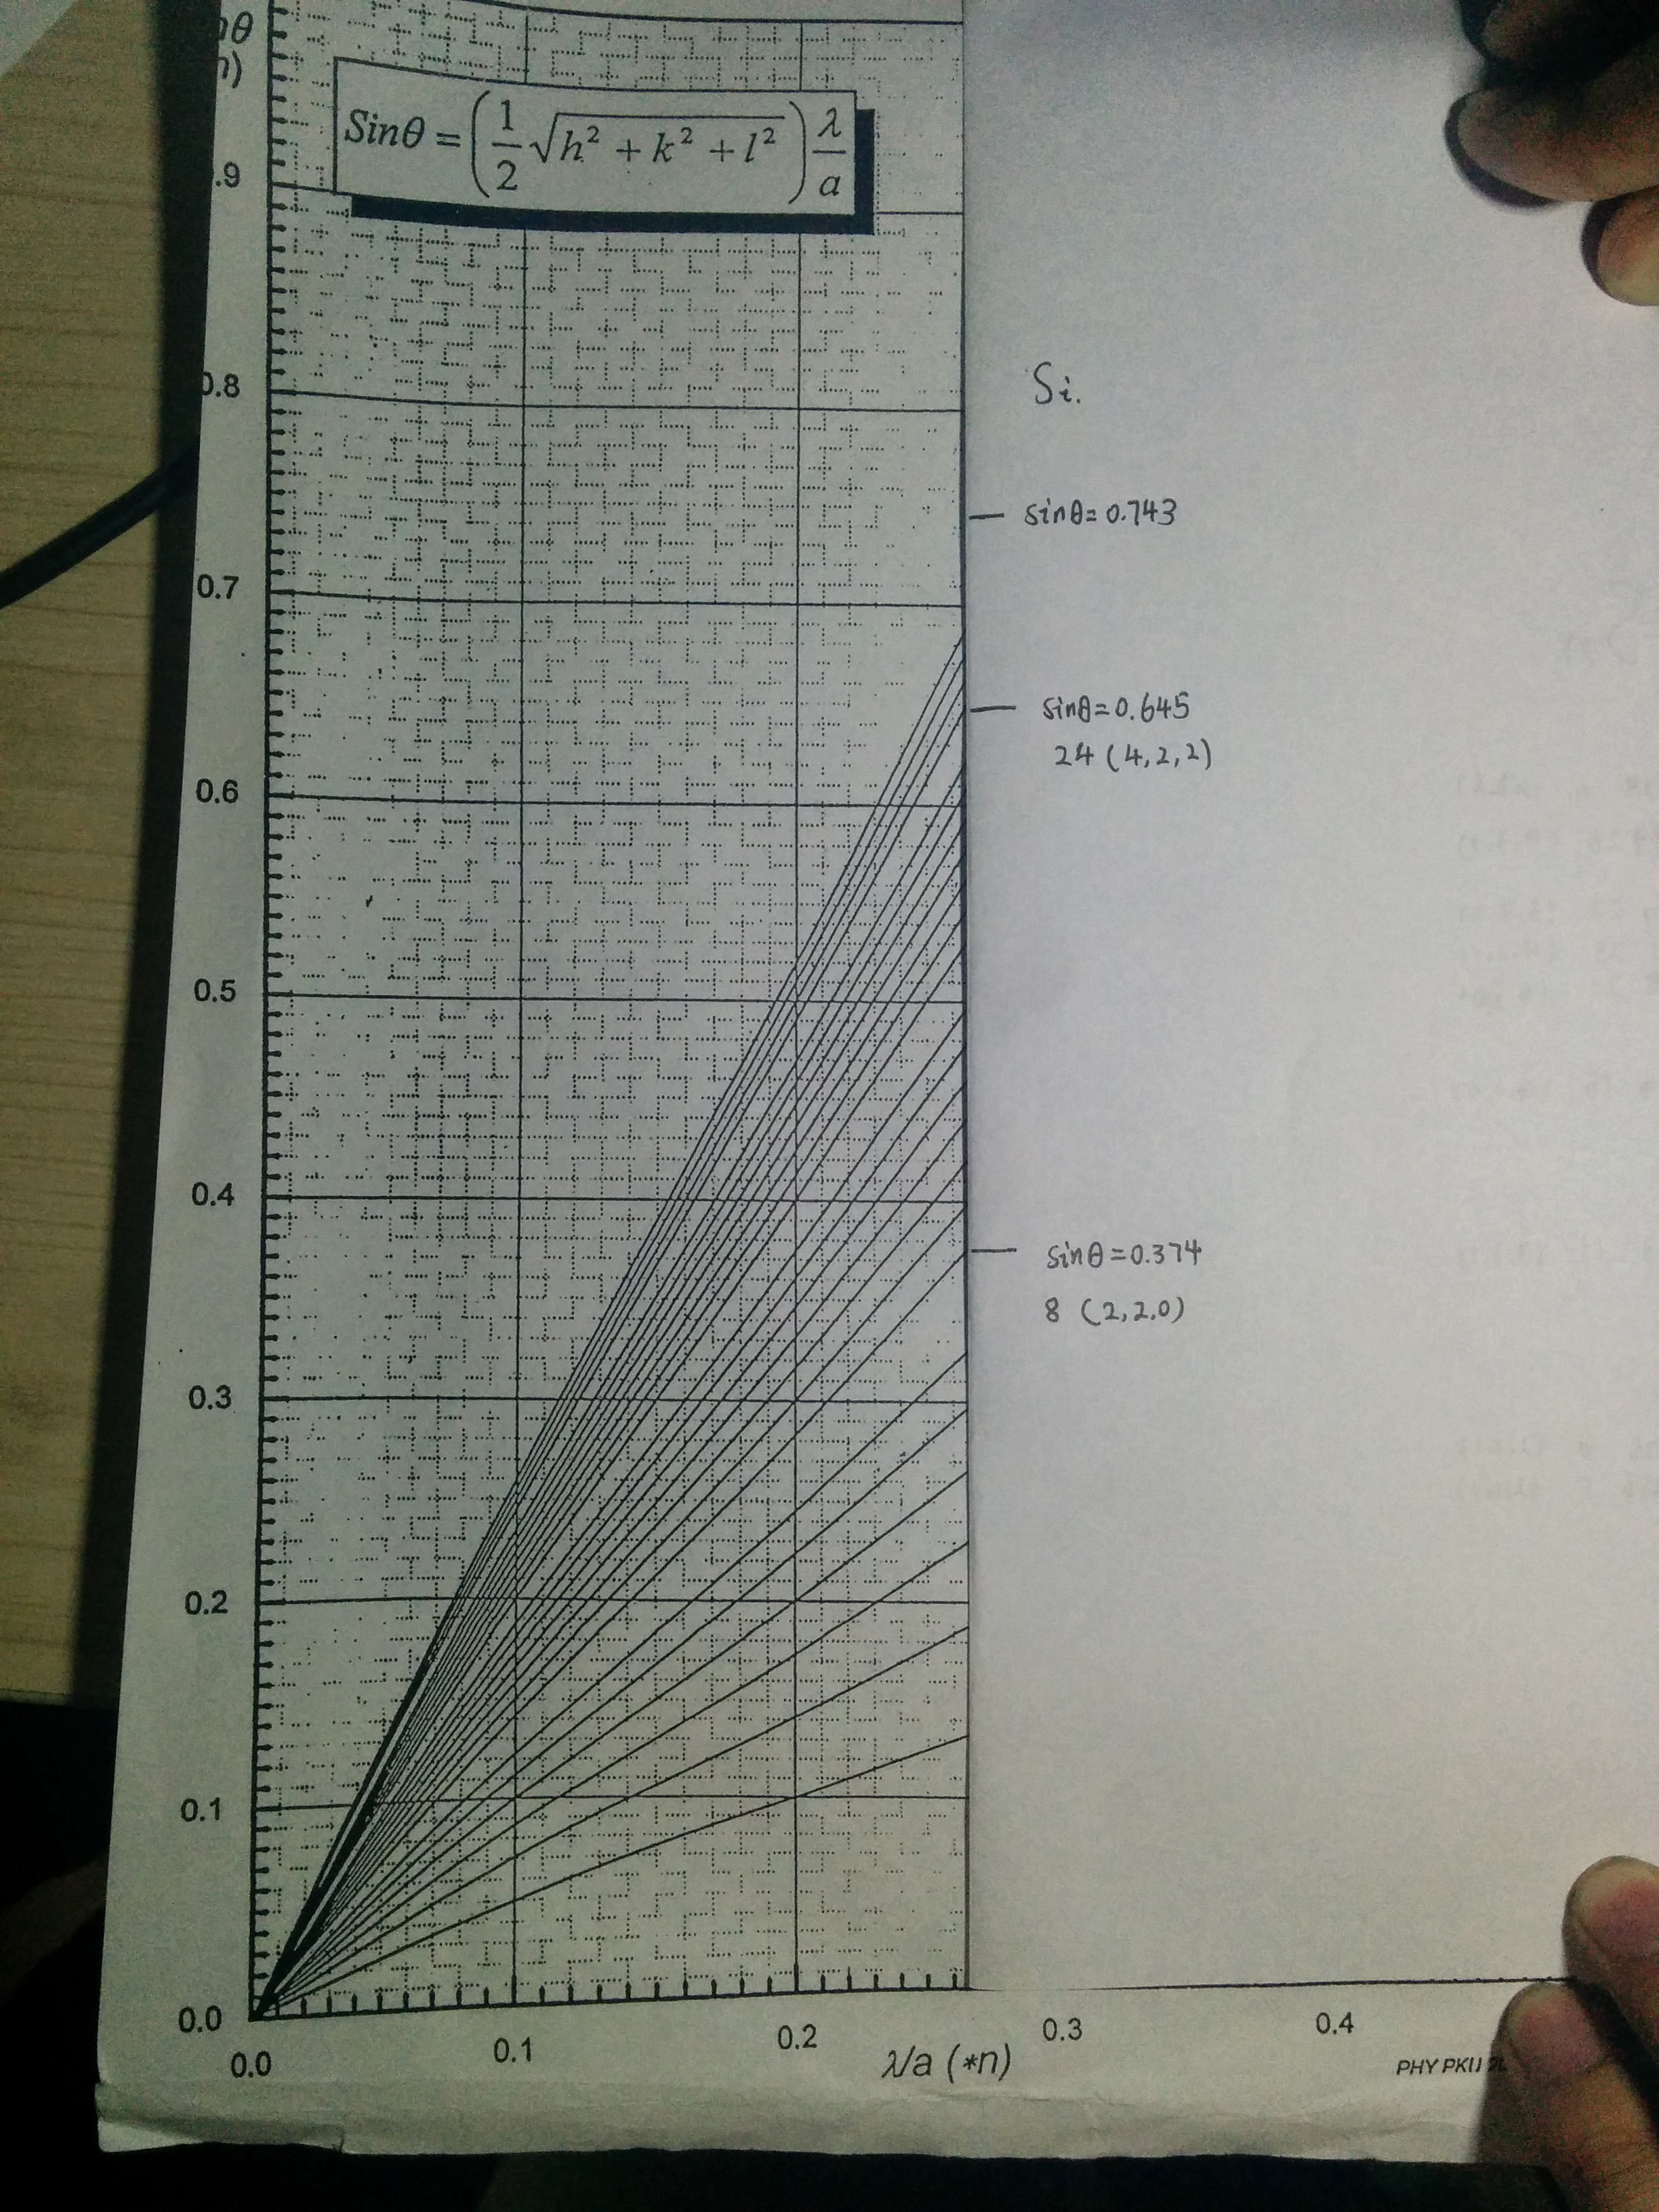
\includegraphics[width=0.55\textwidth]{Si.png}
		\caption{\label{fig:exp2}硅 指标化示意图}
	\end{center}
\end{figure}
\newpage
如图所示可以得到硅的晶格常数满足:
\begin{equation}
	\frac{\lambda}{a_0}=0.263
\end{equation}
从而得到硅的晶格常数为 $a_0=5.7\AA$,其晶面指数组合分别为(2,2,0)和(4,2,2)。硅的数据比较少,所以指标化的时候参照了硅的理论上的晶格常数。

这个实验的误差来源我认为主要来自于指标化过程。可以看出由Au定标引入的误差非常的小,只有千分之五左右。而由于度数引入的误差则有百分之二左右。在指标化过程中,由于刻线之间相互确认完全是一个主观性质的确认,同时因为每一个点都有一定的误差,而指标化过程并不能减少这个误差反而是增加了这个误差,尤其是在出现一些点并不是如预想中的出现在指定的位置而是便宜了一定的位置,这时候指标化确定$\lambda/a$就变的极其的困难了,由主观因素引入的误差就更大了。同时这次进行指标化的纸的直线并不十分的直,可能是因为复印的问题造成的。还有尺子度数和自身精确性的问题使得这个实验的误差变的较大而且很难确定。所以在给出最后的晶格常数的时候我只保留了2位有效数字,以保守一些。

\section{结论}

这个实验通过电子衍射显微镜测量Ag,Cu,Sn,Si的晶格常数。

Ag为多晶体,其晶格常数为$4.1\AA$。

Cu为多晶体,其晶格常数为$3.6\AA$。

Sn为多晶硅,其晶格常数为$6.5\AA$。

Si为单晶体,其晶格常数为$5.7\AA$。


\section{致谢}
感谢季航老师的指导,以及贾春燕,冉书能老师的技术支持。


\begin{thebibliography}{}
	\bibitem{Book} 吴思成,王祖铨~2010 近代物理实验(第三版)(北京:高等教育出版社)第274页.
	\bibitem{guti} 黄昆 固体物理学 (北京:高等教育出版社)
%
%
\end{thebibliography}

\clearpage
\appendix
\section{思考题}

1、两者在几何关系上基本相似,都满足劳厄方程和布拉格公式。X射线和电子都具有波动性质,都具有波长,在物理图像上两者基本一致。不过X射线本身是光子,整体中性不带电,不易受到原子核带电的影响。而电子本身带负电,很容易与核相互作用而造成散射衰弱,所以电子衍射的穿透性很差,样品必须十分的薄才可以。同样的因为散射作用很强以至于衍射的电子束强度和透射的相当,这一点比X光衍射要强很多。同时电子衍射的波长可以很短,衍射角度也很小。

2、因为晶格指数有三个自由度,并且相互是离散的,所以传统的方法很难确定出晶格常数。
其他的方法我认为可以使用电脑来处理指标化,而不是人眼。即和人工处理完全类似,不过是有计算机计算每一个点到距离最近的直线之间的距离的平方和,当这个值最小的时候就可以得到指标化的结果。这样也可以用一定的方法引入误差从而使得研究得到的数据更为可信。

\section{实验记录本}

\begin{figure}[h]
	\begin{center}
		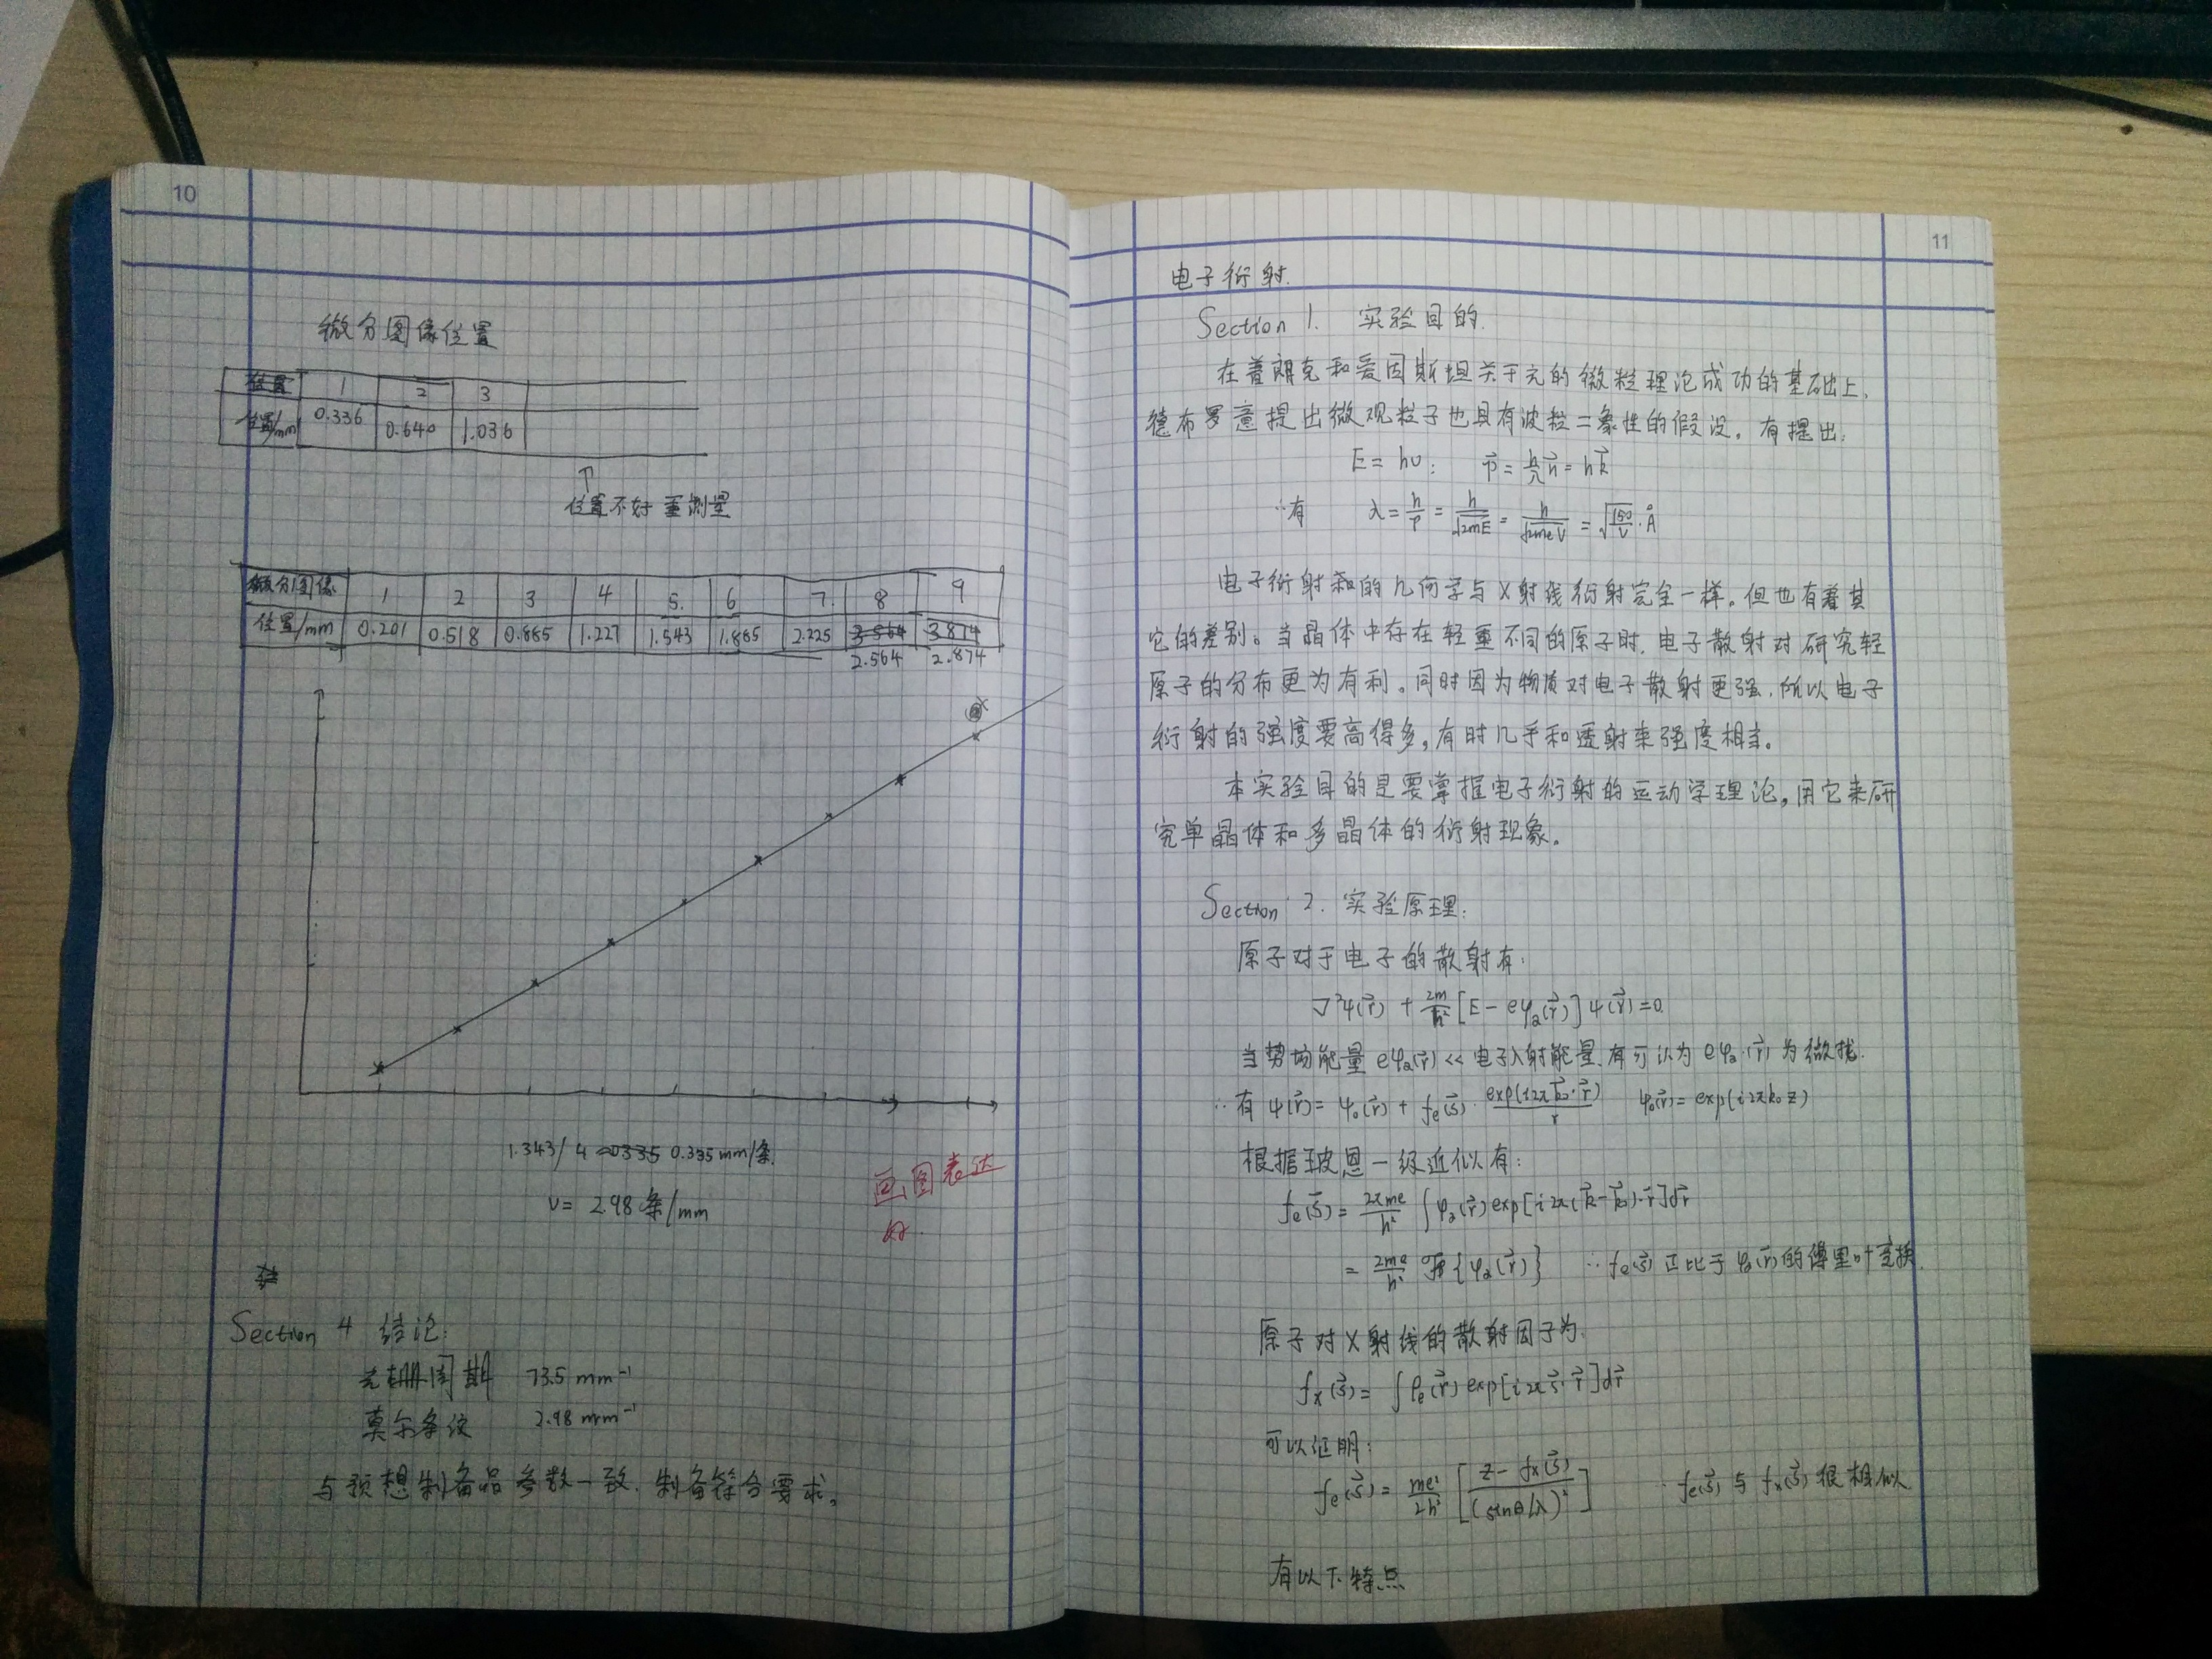
\includegraphics[width=0.8\textwidth]{jiluben1.png}
	\end{center}
\end{figure}
\begin{figure}[h]
	\begin{center}
		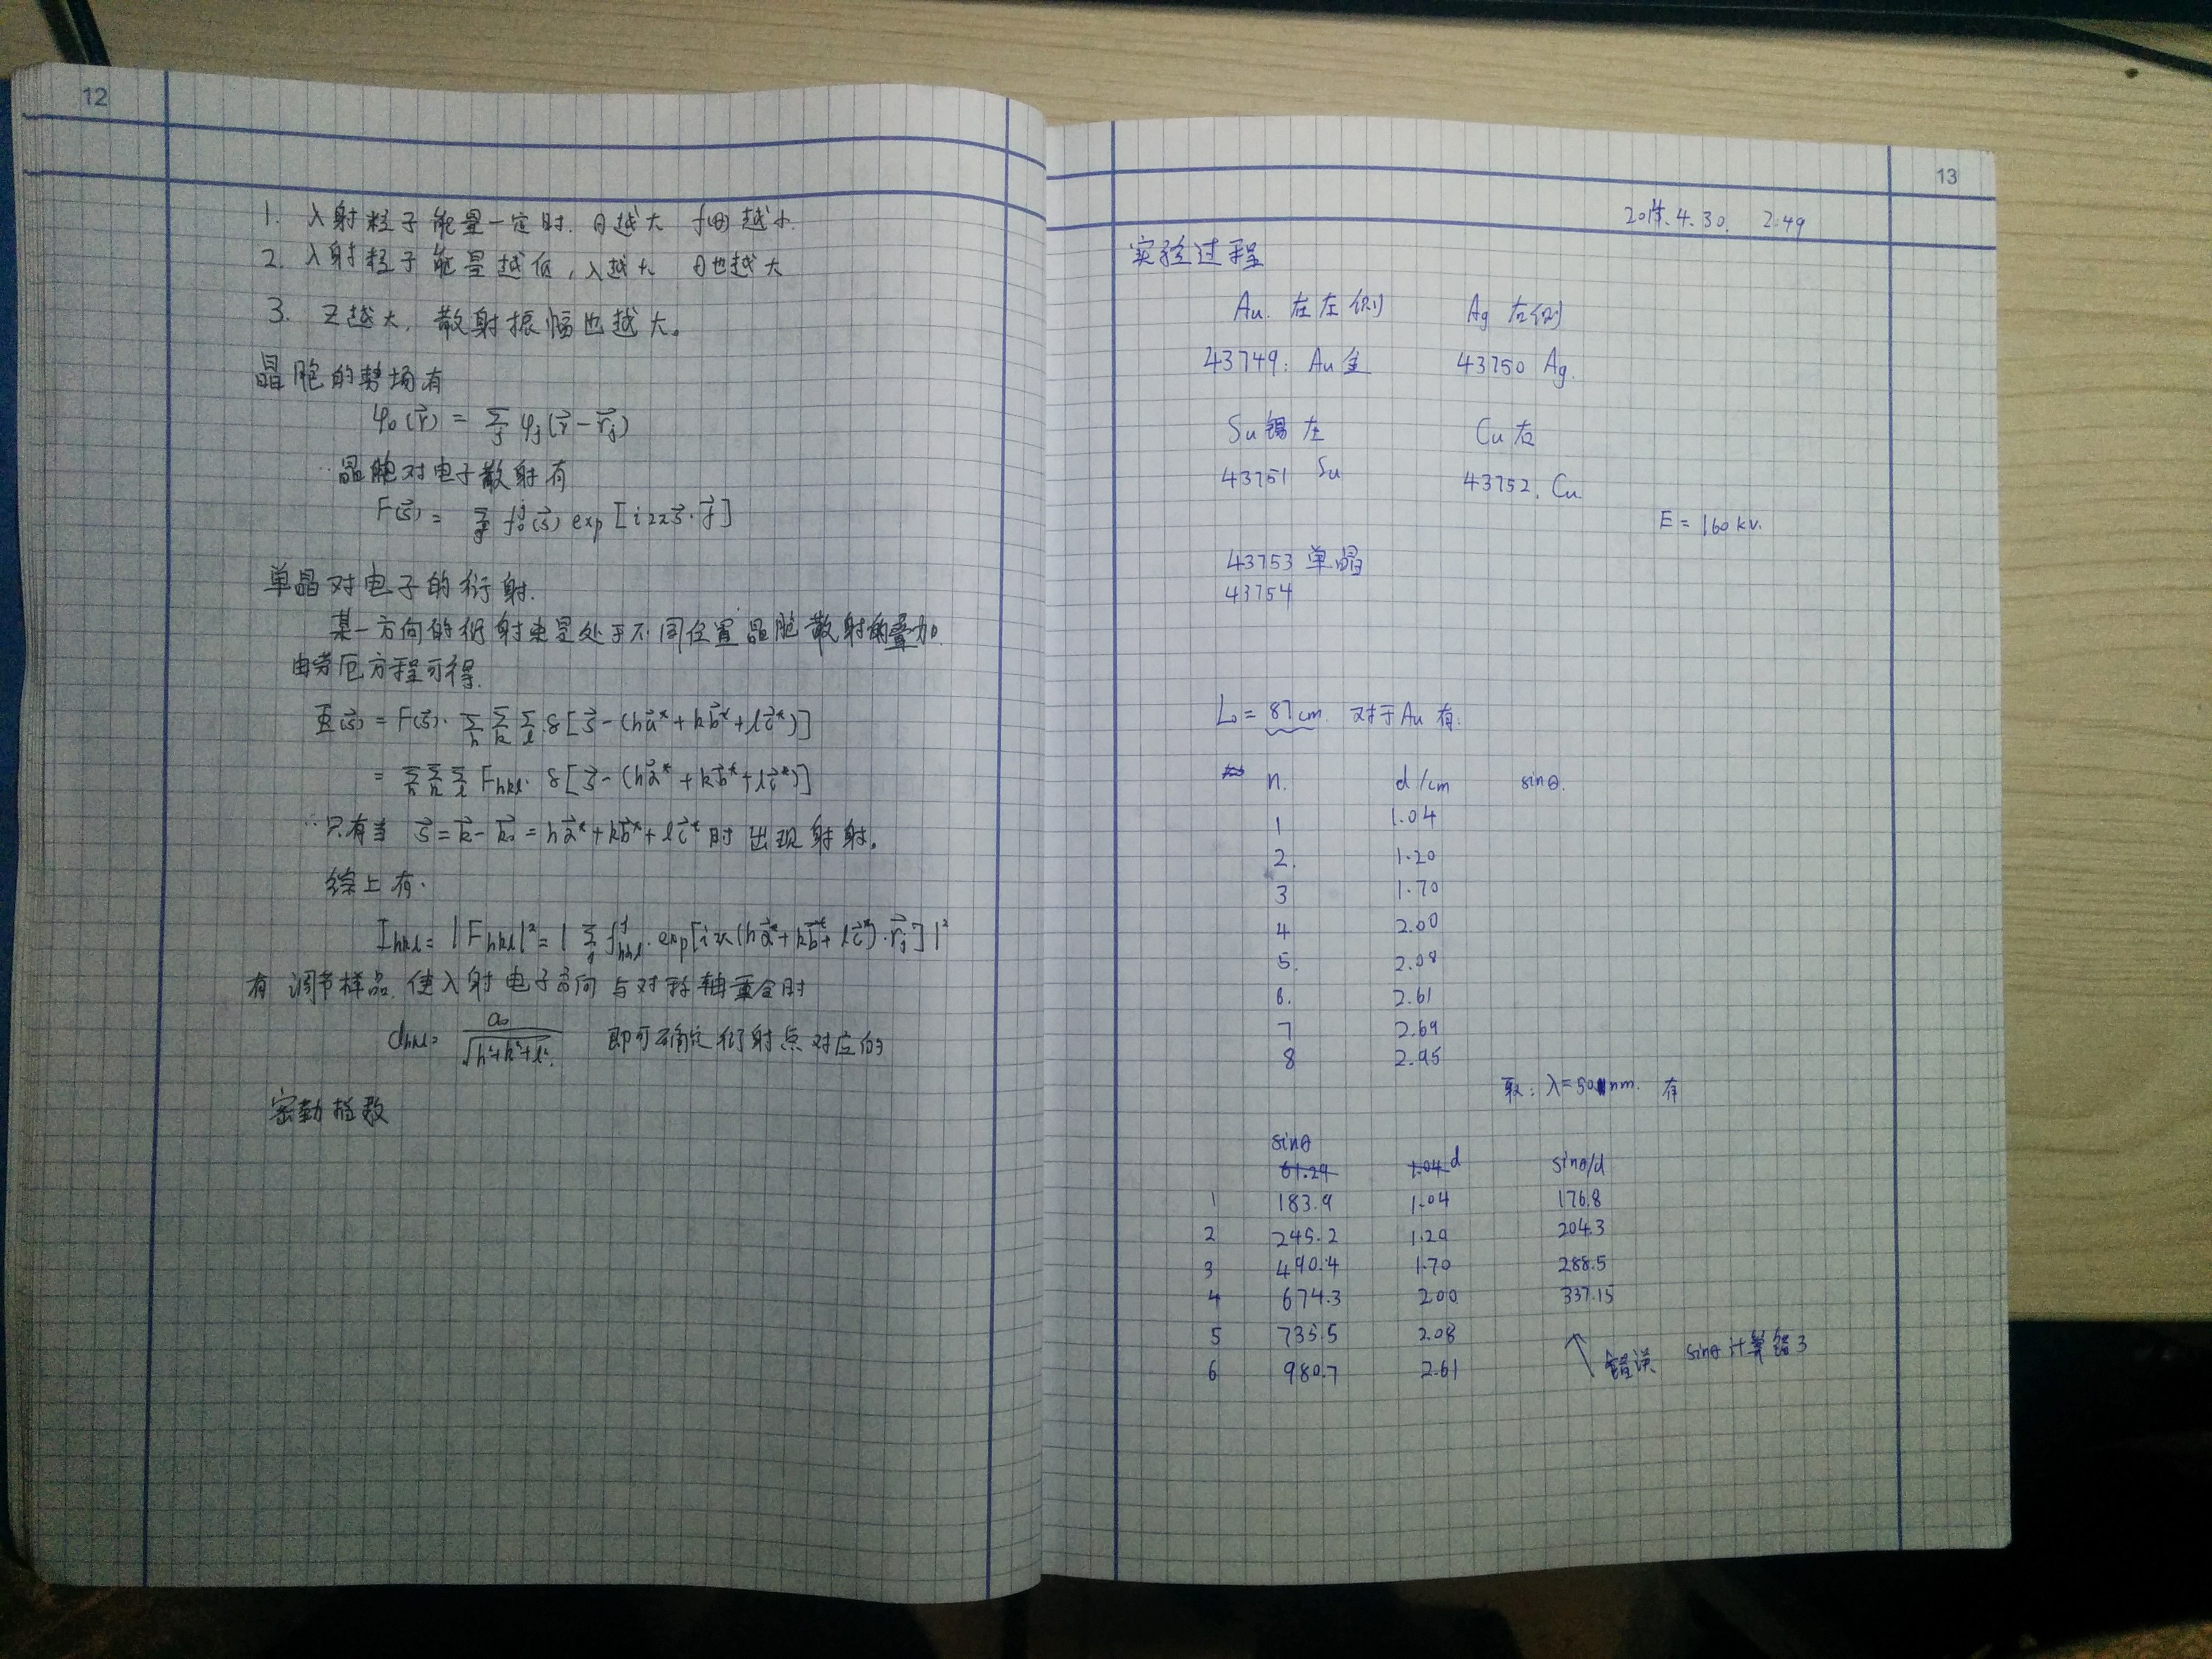
\includegraphics[width=0.8\textwidth]{jiluben2.png}
	\end{center}
\end{figure}
\begin{figure}[h]
	\begin{center}
		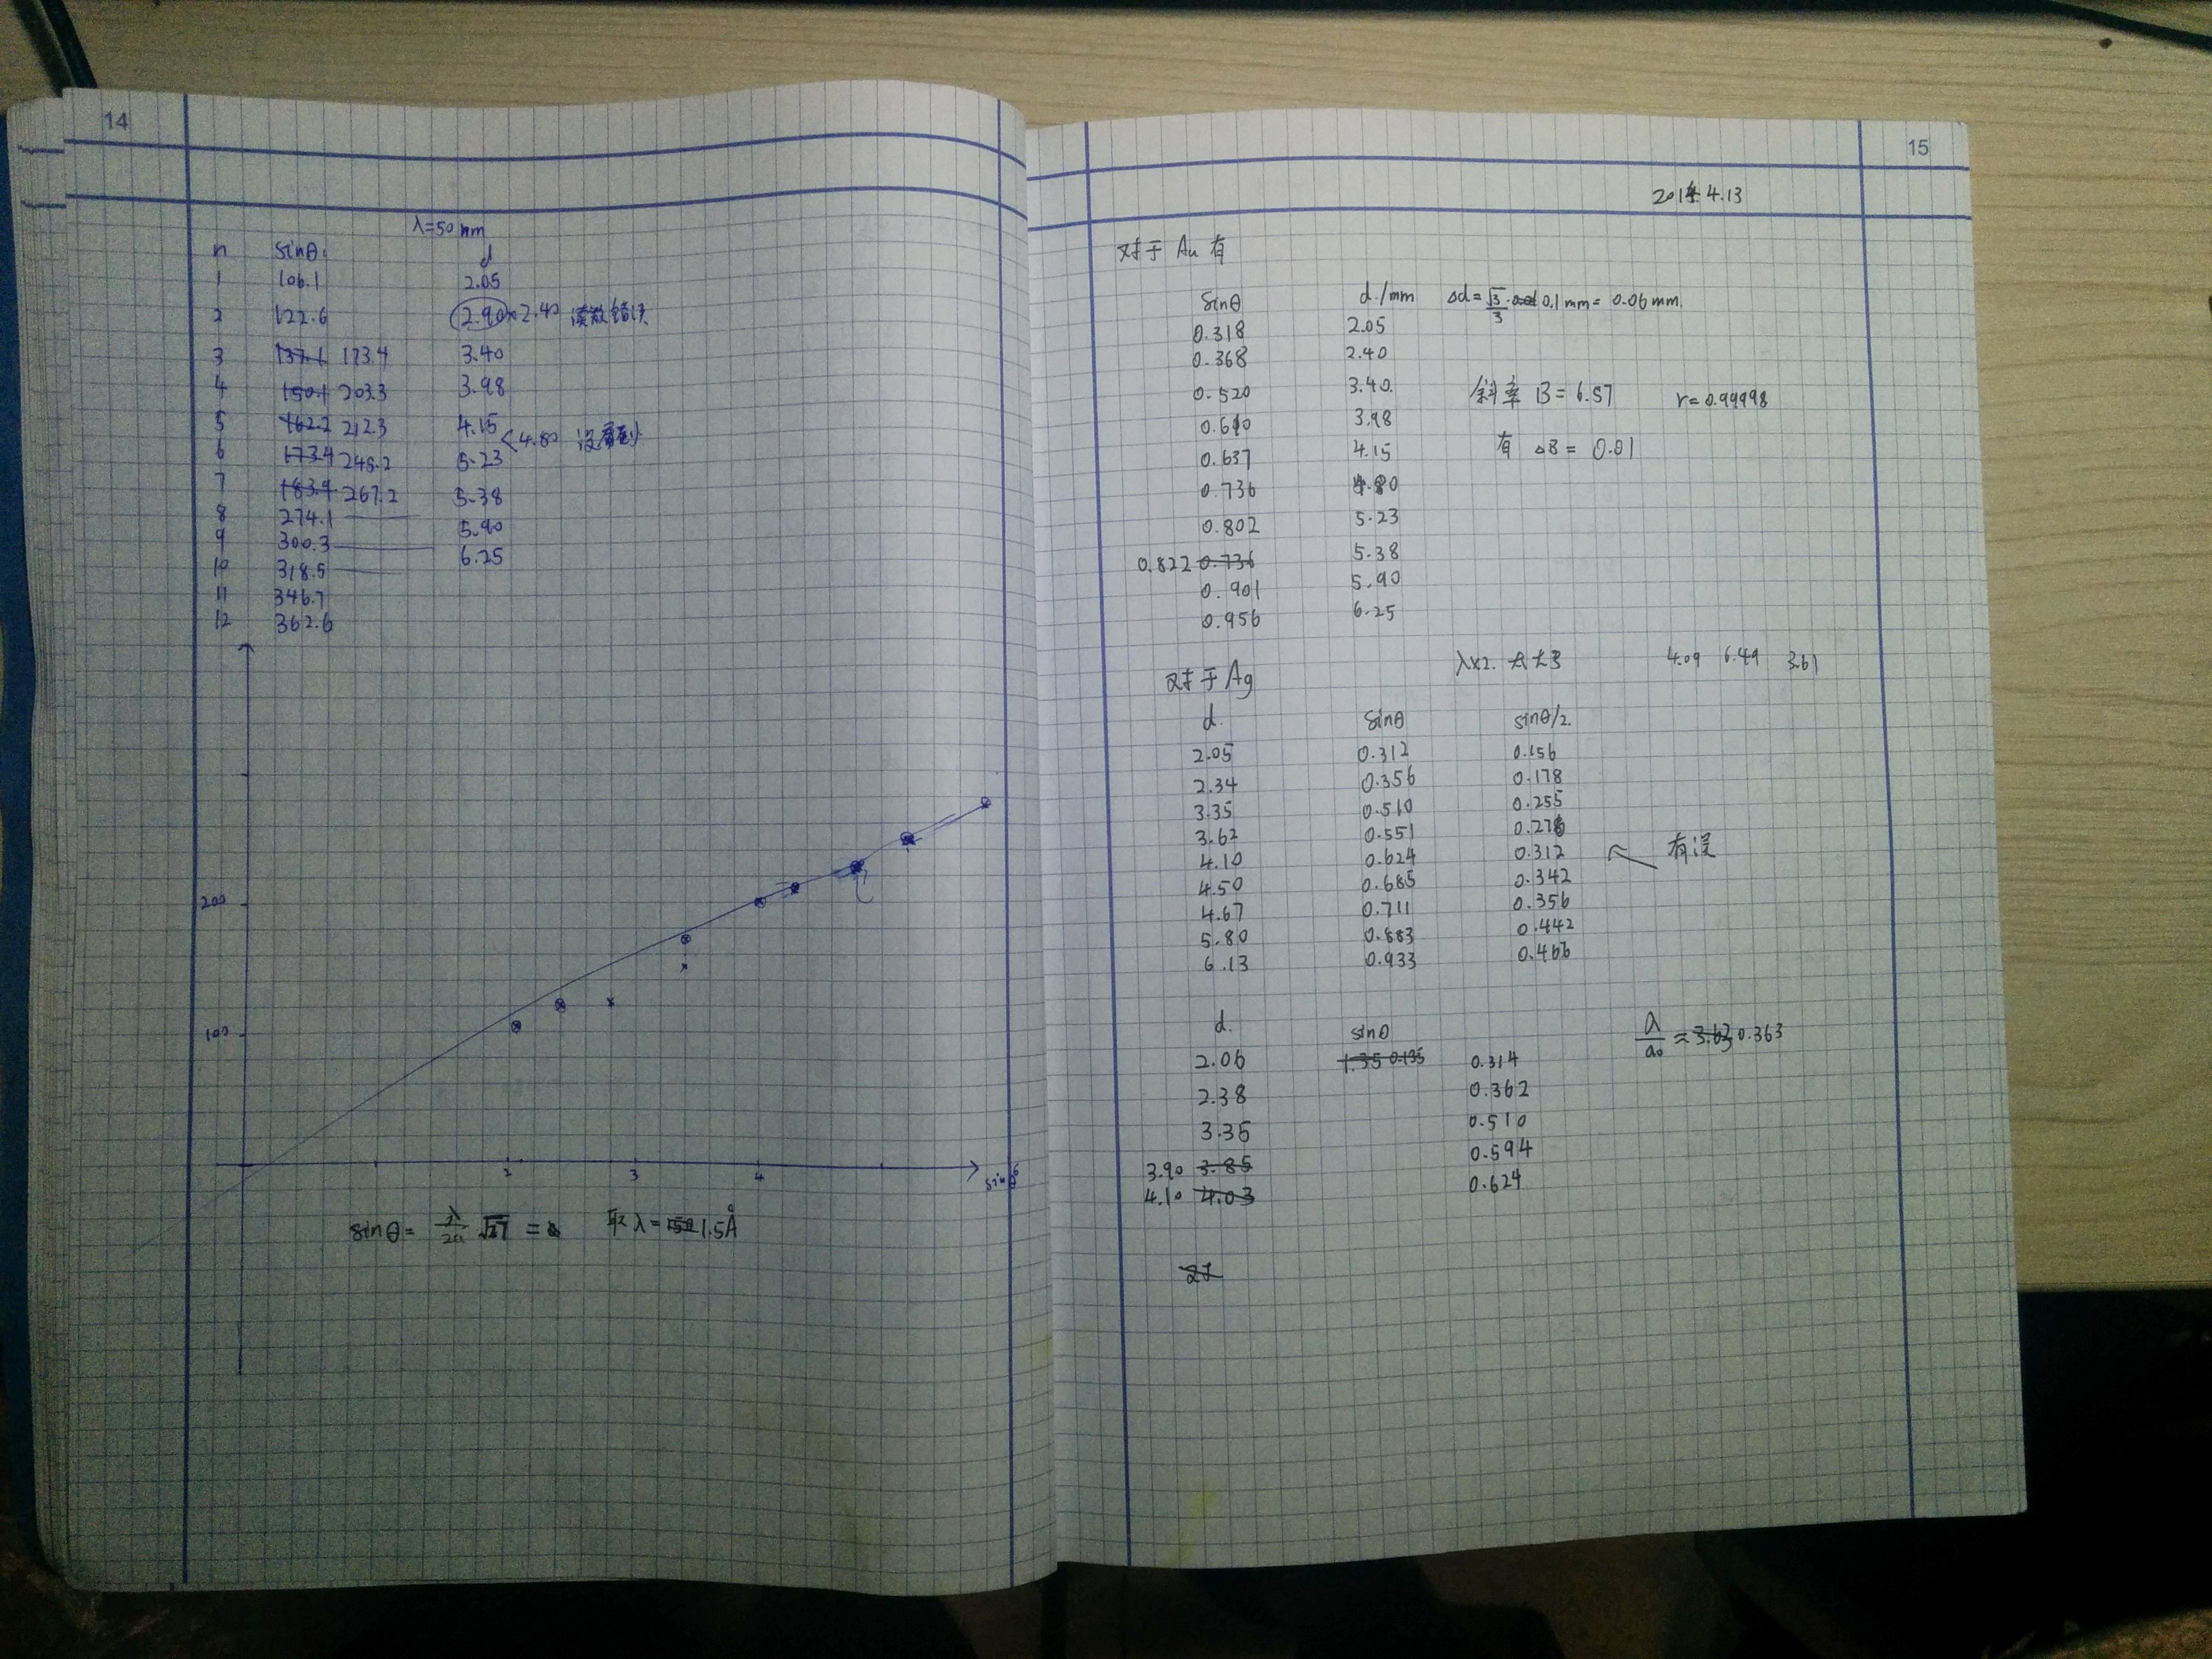
\includegraphics[width=0.8\textwidth]{jiluben3.png}
	\end{center}
\end{figure}
\begin{figure}[h]
	\begin{center}
		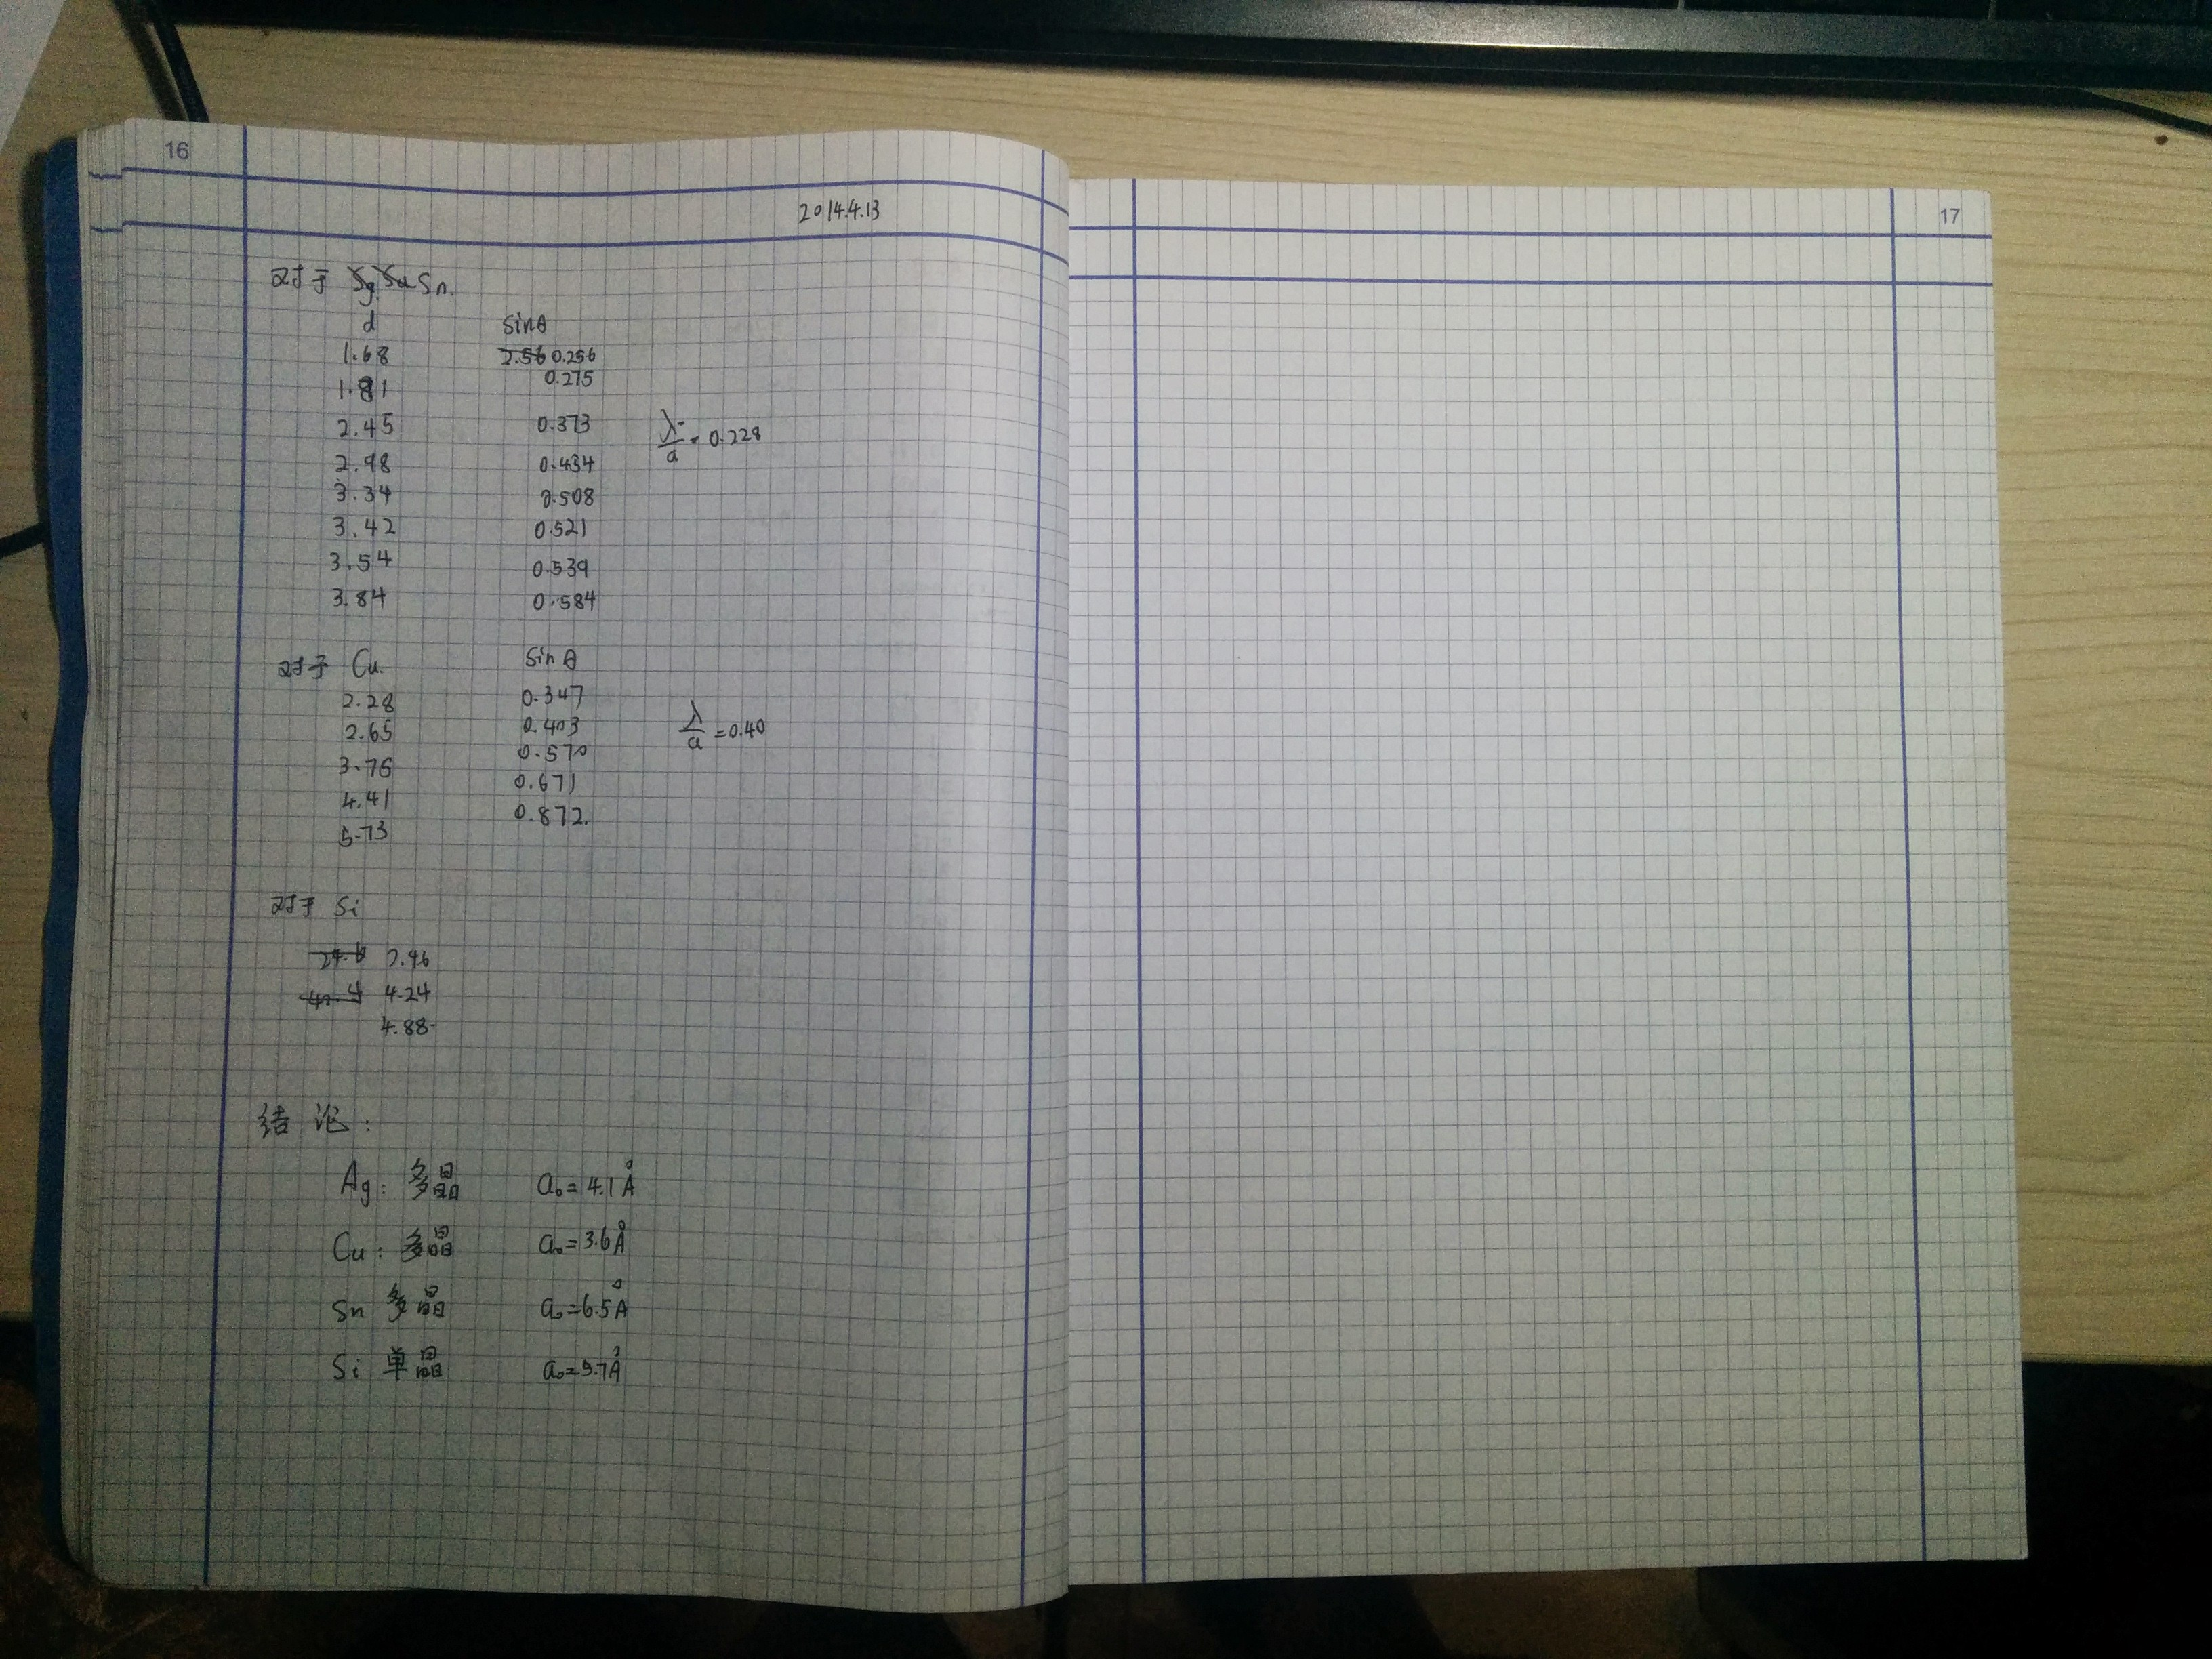
\includegraphics[width=0.8\textwidth]{jiluben4.png}
	\end{center}
\end{figure}


\end{document} 
